\chapter{量子力学}
\originalpage{222}{207}

相比经典力学中的电磁场、温度场、速度场这些时空上的物理量分布，量子力学中的波函数展现了其独特的性质。最鲜明的一点在于，当同时存在多个物理对象时，经典场仅需求解一系列场 $\{\bm E,\bm B,\rho,\bm J,\ldots\}$ 在时空坐标 $\bm r,t$ 下的偏微分方程组，而虽然在量子力学中要求解的函数只有一个（波函数），但它却要从单个时空坐标的函数 $\psi(\bm r,t)$ 转变成多个自变量以及多个下标的一个复杂函数 $\psi_{\sigma\lambda\cdots}(\bm r_1,\bm r_2,\bm r_3,\ldots,t)$。换言之，随着自由度的增长，经典场的复杂度增长是线性的，而对于量子问题则是指数式的。当然，这也是量子计算机具有远胜于经典计算机的潜能的根源。

本章中，我们将首先更进一步讨论单个物理对象的量子系统，然后引入两个甚至多个量子系统间的耦合。在见证了计算复杂度指数增长的维度灾难后，我们也会简要介绍几种近似处理多自由度量子系统的理论。

本章将不会介绍太多数值算法，而是讨论如何将量子力学中的各种实际问题转换成能够用本书其他章节介绍过的算法来求解的形式。

为了行文方便，我们在本章中将始终取 $\hbar=1$。

量子力学的内容涵盖过广，本章所涉及的仅是皮毛。

\section{定态量子系统：微扰论与连续态}

我们在 5.3 节中以氢原子的含时薛定谔方程为例，讨论了如何对其进行分离变量。其中第一步，便是对于满足时间平移不变的含时薛定谔方程
\begin{equation}
 i\partial_t|\Psi\rangle=\hat H|\Psi\rangle
\tag{6.1.1}
\end{equation}
进行分离变量，得到关于哈密顿算符的本征值方程
\begin{equation}
 E|\Psi\rangle=\hat H|\Psi\rangle.
\tag{6.1.2}
\end{equation}
求解哈密顿算符 $\hat H$ 的本征谱 $\{E_i\}$ 是量子力学中的核心问题之一。对于可以分离变量的情形，我们已经了解了如何求解分离得到的一维本征值方程。而如果不能分离变量，直接使用有限元法，或者使用多组一维基函数做直积得到高维的基函数也能够处理。不过，实践中的求解方法远不限于此。此外，为了描述一些实际物理过程，我们也需要超出平方可积这一条限制，例如研究在无穷远处不为零的散射态，甚至于讨论哈密顿算符中虚部不为零的“本征值”。本节中我们将简要介绍一下这些问题。

\subsection{微扰论与本征基组}
\originalpage{223}{208}

对于氢原子问题最简单的推广便是，若外加一个静电场或静磁场，它的本征能量和本征态会怎样变化？此时，它的哈密顿量会具有如下形式：
\begin{equation}
 \hat H(\lambda)=\hat H_0+\lambda\hat H_1,\qquad \lambda\ll1,
\tag{6.1.3}
\end{equation}
其中 $\hat H_1$ 为电偶极或磁偶极相互作用，而参数 $\lambda$ 则正比于外加的电场强度或磁场强度，它通常远小于原子内部的电磁场强度。在量子力学的课程中我们学过，如果已知 $\hat H_0$ 的全体本征对 $\{E_i,|i\rangle\}$，那么 $H(\lambda)$ 的本征对的表达式由下式给出：
\begin{equation}
\begin{aligned}
 E_i(\lambda)&=E_i^{(0)}+\lambda E_i^{(1)}+\lambda^2E_i^{(2)}+\cdots,\\
 |i(\lambda)\rangle&=|i\rangle^{(0)}+\lambda|i\rangle^{(1)}+\lambda^2|i\rangle^{(2)}+\cdots.
\end{aligned}
\tag{6.1.4}
\end{equation}
不过，高阶修正的表达式通常都十分复杂，包含着大量的求和与矩阵向量乘积，对于 $\hat H_0$ 本征值简并的情形，也需要额外处理。而且，幂级数往往也只在某个收敛半径 $|\lambda|<C$ 内才能收敛。

不过，我们可以注意到一个事实，即各阶微扰修正的表达式完全由那些 $\hat H_0$ 的本征态以及哈密顿量在它们间的内积 $\langle i|H_1|j\rangle$ 构成，这提示我们可以用这些本征态作为基组展开波函数：
\begin{equation}
 |\Psi\rangle=\sum_i c_i|i\rangle,
\tag{6.1.5}
\end{equation}
从而得到矩阵形式的本征值方程
\begin{equation}
 \sum_j\bigl(E_i\delta_{ij}+\lambda\langle i|H_1|j\rangle\bigr)c_j=E(\lambda)c_i.
\tag{6.1.6}
\end{equation}
对基组做一个截断，我们便可以通过求解一个矩阵的本征值问题来得到本征谱了。这种方法的计算量与收敛性并不显著依赖于 $\lambda$ 的值，也和系统中是否存在简并无关。

作为一个例子，让我们考虑非谐振子的哈密顿量
\begin{equation}
 \hat H(\lambda)=\frac{p^2+x^2}{2}+\lambda x^4.
\tag{6.1.7}
\end{equation}
当 $\lambda=0$ 时，系统是一个标准的谐振子，能谱为 $E_n=n+\tfrac12$，而本征态可以由升降算符给出：
\begin{equation}
 |n\rangle=\frac{1}{\sqrt{n!}}(\hat a^\dagger)^n|0\rangle.
\tag{6.1.8}
\end{equation}
如果我们将依赖的项视作微扰，使用微扰论，最后得到的结果应当是某个幂级数：
\begin{equation}
 E_n(\lambda)=E_n^{(0)}+\lambda E_n^{(1)}+\lambda^2E_n^{(2)}+\cdots.
\tag{6.1.9}
\end{equation}

\originalpage{224}{209}
注意到，当 $\lambda\to0^-$ 时，系统的势能项 $x^2/2+\lambda x^4$ 是没有下界的：在 $x^2>-1/4\lambda$ 后，势能就会一直下降，直至负无穷。此时系统的基态能量应当也是负无穷。但是，如果 $\lambda$ 从正半轴趋向于零，即 $\lambda\to0^+$，势能项又是有下界的，系统的能谱应当趋向于谐振子的能谱。这个事实说明了 $\lambda=0$ 是函数 $E_n(\lambda)$ 的本性奇点，从而幂级数的收敛半径是零：我们完全没法从微扰论中得到我们所需要的结果。

这时我们就必须求助于数值算法了。以谐振子的本征态作为基组，矩阵元是容易解析计算的：
\begin{equation}
\begin{aligned}
 \langle m|x^4|n\rangle=\frac14\Bigl[&\delta_{m,n+4}\sqrt{(n+1)(n+2)(n+3)(n+4)}\\
 &+\delta_{m,n+2}\sqrt{(n+1)(n+2)}(4n+6)\\
 &+\delta_{m,n}(6n^2+6n+3)\\
 &+\delta_{m,n-2}\sqrt{n(n-1)}(4n-2)\\
 &+\delta_{m,n-4}\sqrt{n(n-1)(n-2)(n-3)}\Bigr].
\end{aligned}
\tag{6.1.10}
\end{equation}
依此我们可以取恰当的截断，对角化矩阵以得到所需的本征能量。

图 6.1 分别给出了微扰论和数值对角化得到的基态能量随参数 $\lambda$ 的变化关系。(a) 图为微扰阶数分别从 0 取到 4 的结果。可以看出，随着微扰论阶数的升高，计算结果无法收敛，这来源于前面提及的收敛半径为零。(b) 图为截断 $n_{\max}$ 分别为 0, 2, 4, 6 的结果。$n=0$ 与一阶微扰论等价（请读者思考一下原因），而当 $n_{\max}\ge4$ 时，肉眼就已经几乎无法区分不同截断之间的差别了，结果收敛得非常快。

\begin{figure}[htbp]
\centering
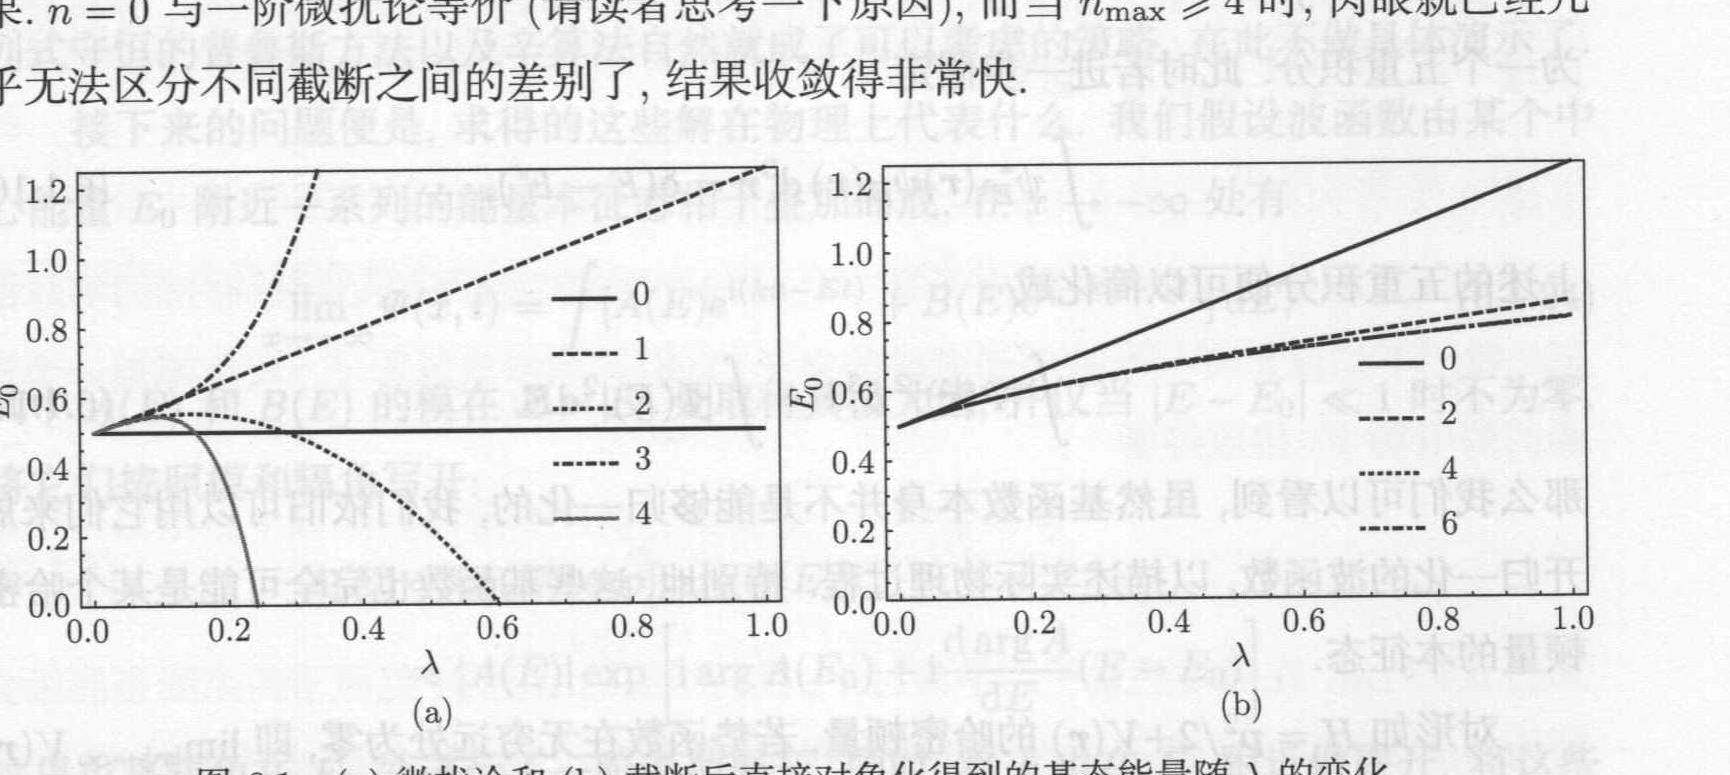
\includegraphics[width=.92\linewidth]{figures/fig6_1_anharmonic.png}
\caption{(a) 微扰论和 (b) 截断后直接对角化得到的基态能量随 $\lambda$ 的变化}
\label{fig:6-1}
\end{figure}

与之类似的问题也出现在量子场论的Feynman 图展开中：将所有阶数的树图和圈图加起来，结果通常是发散的。尽管解析上也存在诸如重求和等处理办法，但展开中存在发散行为也是人们希望通过格点场论直接数值求解量子场论问题的动机之一。

\originalpage{225}{210}
\begin{exerciseBox}[练习 6.1]
请尝试自行推导 (6.1.10) 式。读者可以查阅量子力学教材获知升降算符的性质。
\end{exerciseBox}

\subsection{连续谱与散射态}

在量子力学中，我们总是要求描述实际物理系统的波函数是平方归一的：
\begin{equation}
 \int |\Psi|^2\,\mathrm d^3r=1,
\tag{6.1.11}
\end{equation}
因此，我们也会同时期待用以展开波函数的基组是平方可积的：
\begin{equation}
 \int |\psi_i|^2\,\mathrm d^3r<\infty,
\tag{6.1.12}
\end{equation}
否则表达式
\begin{equation}
 \int\left|\sum_i c_i\psi_i\right|^2\mathrm d^3r
\tag{6.1.13}
\end{equation}
中就会包含一些无穷大的求和，与归一化的条件相冲突。但这件事也不尽然，如果基函数不是以离散的角标 $i$ 来分别，而是以某个连续的变量 $E$ 描述，那么此时有
\begin{equation}
 \Psi(\bm r)=\int \Phi(E)\psi_E(\bm r)\,\mathrm dE,
\tag{6.1.14}
\end{equation}
以及
\begin{equation}
 \int|\Psi(\bm r)|^2\,\mathrm d^3r
 =\int \Phi^*(E')\Phi(E)\psi_{E'}^*(\bm r)\psi_E(\bm r)\,\mathrm d^3r\,\mathrm dE\,\mathrm dE',
\tag{6.1.15}
\end{equation}
为一个五重积分。此时若进一步假定
\begin{equation}
 \int \psi_{E'}^*(\bm r)\psi_E(\bm r)\,\mathrm d^3r=\delta(E-E'),
\tag{6.1.16}
\end{equation}
上述的五重积分便可以简化成
\begin{equation}
 \int|\Psi(\bm r)|^2\,\mathrm d^3r=\int|\Phi(E)|^2\,\mathrm dE.
\tag{6.1.17}
\end{equation}
那么我们可以看到，虽然基函数本身并不是能够归一化的，我们依旧可以用它们来展开归一化的波函数，以描述实际物理过程。特别地，这些基函数也完全可能是某个哈密顿量的本征态。

对形如 $H=p^2/2+V(\bm r)$ 的哈密顿量，若势函数在无穷远处为零，即 $\lim_{|\bm r|\to\infty}V(\bm r)\to0$，那么可以断定，$H$ 能量为 $E>0$ 的本征函数在 $|\bm r|\to\infty$ 处一定具有 $\exp(i\bm k\cdot\bm r)$ 的形式，其中 $k^2=2E$。特别地，对于一维问题有
\begin{equation}
 \psi_E(x)=
 \begin{cases}
 Ae^{ikx}+Be^{-ikx},&x\to-\infty,\\
 Ce^{ikx}+De^{-ikx},&x\to\infty.
 \end{cases}
\tag{6.1.18}
\end{equation}

\originalpage{226}{211}
(6.1.18) 式中的 $A,B,C,D$ 四个系数自然不可能是独立的。原则上讲，如果给定了 $A$ 和 $B$，我们就获知了 $x=-\infty$ 处的边界条件。通过求解二阶线性齐次常微分方程
\begin{equation}
 -\frac12\psi''+V\psi=E\psi
\tag{6.1.19}
\end{equation}
的初值问题，可以得到 $\psi_E(x)$ 的完整形式，从而确定系数 $C$ 和 $D$ 值。由于问题是线性的，有矩阵形式
\begin{equation}
 \begin{pmatrix}C\\D\end{pmatrix}
 =\begin{pmatrix}T_{11}&T_{12}\\T_{21}&T_{22}\end{pmatrix}
 \begin{pmatrix}A\\B\end{pmatrix}.
\tag{6.1.20}
\end{equation}
我们可以进一步讨论转移矩阵 $\mathbf T$ 会满足什么条件。首先，这个二阶微分方程具有 SL 型方程 (5.3.8) 的形式，并且 $p(x)$ 是一个常数。从而根据 (5.3.14) 式，Wronski 行列式
\begin{equation}
 W[f,g](x)=gf'-fg'
\tag{6.1.21}
\end{equation}
是守恒量，其中 $f(x)$ 和 $g(x)$ 是能量相同的定态。我们令 $g=f^*$，此时Wronski 行列式 $W[f,f^*]$ 等价于量子力学中引入的概率流。取 $x=\pm\infty$，可以得到
\begin{equation}
 |A|^2-|B|^2=|C|^2-|D|^2.
\tag{6.1.22}
\end{equation}
由于上式对任意的 $A$ 和 $B$ 均成立，再借助 (6.1.20) 式，可证明转移矩阵 $\mathbf T$ 满足
\begin{equation}
 \mathbf T^\dagger
 \begin{pmatrix}1&0\\0&-1\end{pmatrix}
 \mathbf T=
 \begin{pmatrix}1&0\\0&-1\end{pmatrix}.
\tag{6.1.23}
\end{equation}
我们自然希望数值求解得到的转移矩阵同样满足概率流守恒，此时能够保证Wronski 行列式守恒的辛算法以及辛算法自然就成了可以考虑的策略，在此不做具体演示了。

接下来的问题便是，求得的这些解在物理上代表什么，我们假设波函数由某个中心能量 $E_0$ 附近一系列的能量本征态相干叠加而成，在 $x\to-\infty$ 处有
\begin{equation}
 \lim_{x\to-\infty}\Psi(x,t)=\int\bigl[A(E)e^{i(kx-Et)}+B(E)e^{i(-kx-Et)}\bigr]\,\mathrm dE,
\tag{6.1.24}
\end{equation}
其中 $A(E)$ 和 $B(E)$ 的模在 $E=E_0$ 处取得其极大值，并仅当 $|E-E_0|\ll1$ 时不为零。将它们按照模和辐角写开：
\[
 A(E)=|A(E)|\exp[i\arg A(E)]
 \approx |A(E)|\exp\left[i\arg A(E_0)+i\frac{\mathrm d\arg A}{\mathrm dE}(E-E_0)\right],
\]
这里也将辐角在 $E_0$ 处进行了一阶Taylor 展开。同时，将 $k$ 也在 $E_0$ 附近做展开。将这些结果代回原积分式，有
\begin{align}
 \lim_{x\to-\infty}\Psi(x,t)\sim{}&e^{i(k_0x-E_0t)}\int e^{i[\frac{\mathrm d\arg A}{\mathrm dE}+\frac{\mathrm dk}{\mathrm dE}x-t](E-E_0)}|A(E)|e^{i\arg A(E_0)}\,\mathrm dE\notag\\
 &+e^{i(-k_0x-E_0t)}\int e^{i[\frac{\mathrm d\arg B}{\mathrm dE}-\frac{\mathrm dk}{\mathrm dE}x-t](E-E_0)}|B(E)|e^{i\arg B(E_0)}\,\mathrm dE.
\tag{6.1.25}
\end{align}

\originalpage{227}{212}
被积函数为一个尖锐的单峰函数乘上一个快速振荡的复指数。通常，仅当振荡频率接近于零时，积分才会有显著的非零值。这分别对应着
\begin{equation}
 x=\frac{\mathrm dE}{\mathrm dk}(t-t_A),\qquad
 x=-\frac{\mathrm dE}{\mathrm dk}(t-t_B),
\tag{6.1.26}
\end{equation}
其中 $t_X\equiv\mathrm d\arg X/\mathrm dE$。我们可以将它们想象成两个波包：$A$ 波包从 $x=-\infty$ 处以速度 $v_g=\mathrm dE/\mathrm dk$ 向前运动，预计在 $t_A$ 时刻到达 $x=0$ 处；而 $B$ 波包则像是一个由 $t=t_B$ 时刻从 $x=0$ 处出发向负半轴处运动的波包，在 $x\to-\infty$ 时具有速度 $v_g$。这里的 $v_g$ 被称为群速度，与哈密顿系统中的广义速度 $\dot q=\partial H/\partial p$ 的定义是一致的。值得注意的是，仅当 $t$ 足够小时我们才能找到波包 $A$，$t$ 足够大时我们才能找到波包 $B$。

对 $x\to\infty$ 处的分析是一致的。由此我们可以设想一个特殊的情景：$A=0$。这意味着在 $t\to-\infty$ 时，波包 $D$ 自 $x=\infty$ 处向原点运动，而在 $t\to\infty$ 时，波包 $B$ 和 $C$ 自原点分别向两端背向而行。我们可以认为，波包 $B$ 就是初始的波包 $D$ 穿过势场 $V(x)$ 的透射波，而波包 $C$ 则是相应的反射波。$B/D=T_{22}^{-1}$ 和 $C/D=T_{12}/T_{22}$ 给出了透射系数和反射系数，而
\begin{equation}
 t_B-t_D=-\frac{\mathrm d}{\mathrm dE}\arg T_{22},\qquad
 t_C-t_D=\frac{\mathrm d}{\mathrm dE}(\arg T_{12}-\arg T_{22})
\tag{6.1.27}
\end{equation}
则可以理解成波包穿过势场和返回所需要的额外时间。将这个时间与经典力学的结果做对比，尤其是在势场中存在经典禁戒区域的时候，是尤为有趣的。

对于二维或更高维度的情形，由于波包的运动不再限于前后两个方向，分析会更困难一些，但基本思想是一致的。

\subsection{复本征能量}

在无穷远处（$|\bm r|\to\infty$）趋向于零 $[V(\infty)=0]$ 的势场远不足以描述全部的实际情形。我们不妨设想有一个被质子束缚的电子，它们共同形成氢原子。现在施加一个微弱的静电场 $\bm F$，构成势场
\begin{equation}
 V(\bm r)=-\frac1r-\bm r\cdot\bm F,
\tag{6.1.28}
\end{equation}
如图 6.2 所示。在通常的量子力学教材中，我们学到的结论是，氢原子的束缚态能级会因为静电场的存在产生一个直流 Stark 能移（DC Stark shift）。然而，不管静电场多弱，当原子和电子的相对位矢 $\bm r$ 足够大时，库仑势总是可以被忽略而仅剩下 $-\bm r\cdot\bm F$，可以趋向于负无穷。那么，氢原子的束缚态波函数原则上是可以越过经典势垒，隧穿到无穷远，成为在电场中做加速运动的准自由粒子的。事实上，对于这个问题，我们根本找不到可归一化的定态：波函数在 $-\bm r\cdot\bm F\to-\infty$ 处总会发散。

\originalpage{228}{213}
\begin{figure}[htbp]
\centering
\begin{tikzpicture}[x=1.1cm,y=1.0cm]
  \draw[->] (-0.2,0) -- (7.2,0) node[below] {$x$};
  \draw[->] (0,0) -- (0,4.2) node[left] {$V(x)$};
  \draw[dashed] (0.15,1.15) -- (6.65,1.15);
  \draw[thick,smooth] plot coordinates {(0.2,3.7) (0.55,3.0) (0.8,2.0) (1.0,0.2) (1.35,-0.6) (1.7,0.4) (2.05,1.1) (2.45,1.55) (3.1,1.78) (3.8,1.72) (4.5,1.53) (5.2,1.25) (5.8,1.0) (6.5,0.55)};
  \node[below] at (2.15,1.12) {$x_i$};
  \node[below] at (5.15,1.12) {$x_f$};
\end{tikzpicture}
\caption{理想无穷大范围静电场作用下的氢原子势场（取沿静电场方向的一维分布）}
\label{fig:6-2}
\end{figure}

找不到可归一化的定态也不一定是个了不得的大难题，无穷大范围内均匀电场在现实中并不可能存在。当跨过用以产生静电场的平行极板后，(6.1.28) 式便无法正确描述势场分布了，在真正的无穷远处，势函数还是会趋向于零。而这个体系实际的基态，应当是电子和质子分别被吸附到正极和负极附近。

但这个实际的基态并不能提供任何有意义的信息：我们所施加的电场也不是什么真正的静电场，而仅仅持续一段时间，这段时间并不足以让氢原子从无外场的基态演化到有外场的“实际基态”。我们更感兴趣的事情是，在电场作用下，单位时间内有多大比例的电子能够脱离库仑势的束缚，变成自由电子？换言之，我们希望能求得隧穿速率 $\Gamma$。在“实际势场”下求解这个问题原则上是可行的，但这意味着我们需要根据具体的实验细节设定远处的势场行为，并在一个相当大的空间中求解波函数。显然，这些实验细节不应当对 $\Gamma$ 造成多大的影响，我们依旧希望在 (6.1.28) 式的框架下来求解问题。

我们从隧穿速率的基本概念出发。处在基态上的电子在单位时间内有 $\Gamma$ 的概率离开基态，这意味着基态布局 $\rho(t)\equiv|\langle g|\Psi(t)\rangle|^2$ 会满足方程
\begin{equation}
 \frac{\mathrm d\rho(t)}{\mathrm dt}=-\Gamma\rho(t).
\tag{6.1.29}
\end{equation}
从中可以解出 $t$ 时刻波函数依旧留在束缚态 $|g\rangle$ 的概率为
\begin{equation}
 |\langle g|\Psi(t)\rangle|^2=e^{-\Gamma t}|\langle g|\Psi(0)\rangle|^2,
\tag{6.1.30}
\end{equation}
呈指数下降。这意味着
\begin{equation}
 |\Psi(t)\rangle\sim e^{-\Gamma t/2}e^{-iEt}|\Psi(0)\rangle\sim e^{-i(E-i\Gamma/2)t}|\Psi(0)\rangle.
\tag{6.1.31}
\end{equation}
\footnote{对于“实际势场”，隧穿后的电子运动至正极板后可能会发生弹性碰撞，经过相当长的时间后再次返回原子核。这对应于波函数等于能量非常接近的若干个束缚态的线性叠加，不过我们通常不会关心这个时间尺度上的行为。}

\originalpage{229}{214}
我们看到，波函数的含时演化似乎可以用一个具有复本征能量的定态来描述！

这着实是一个违背常理的事情，引入静电场后薛定谔方程依旧是时间平移不变的，可以通过分离变量转换成定态薛定谔方程求解本征值问题，而厄米的哈密顿量本征值又只能是实数，这复数是从哪里来的呢？

问题出在了哈密顿量的“厄米性”上。当我们考察在一维静电场中做加速运动的粒子时，由量子力学中所学的 WKB 近似，其波函数
\begin{equation}
 \psi(x)\sim\frac1{\sqrt p}\exp\left(i\int p\,\mathrm dx\right),
\tag{6.1.32}
\end{equation}
其中经典动量
\begin{equation}
 p\equiv\sqrt{2[E-i\Gamma/2-V(x)]}
 \approx\sqrt{2[E-V(x)]}-\frac{i\Gamma}{2\sqrt{2[E-V(x)]}}
\tag{6.1.33}
\end{equation}
的虚部小于零，从而波函数在无穷远处是发散的。而我们仅对于平方可积的函数证明了哈密顿算符的厄米性，那么得到存在一个复本征能量也就不那么奇怪了。

此外，波函数在无穷远处指数发散这件事也不稀奇。积分式
\begin{equation}
 i\int\frac{-i\Gamma}{2\sqrt{2[E-V(x)]}}\,\mathrm dx=\frac\Gamma2t_c
\tag{6.1.34}
\end{equation}
给出了一个经典粒子从原点运动到 $x$ 处的时间 $t_c$。而在 $t-t_c$ 时刻，原点外的波函数幅值应当是 $t$ 时刻波函数幅值的 $\exp(\Gamma t_c/2)$ 倍：波函数在空间无穷远处发散正好对应了其在时间无穷远的过去发散。

解释了合理性，下一个问题是数值上怎么求解。我们以往处理过的问题要么局限在有限区间，要么在无穷远处趋向于零。而临这类发散的问题，只能考虑能否将其转换成一个不发散的问题。幸运的是，这样的转换是存在的。以一维情形为例，对于波函数 $\psi(x)$，我们若不局限于实轴 $\mathbb R$，而将其视作复平面 $\mathbb C$ 上的解析函数，那么在射线 $\arg z=\alpha$ 上，有
\begin{equation}
 \psi(e^{i\alpha}x)\sim\frac1{\sqrt p}\exp\left(ie^{i\alpha}\int p\,\mathrm dx\right).
\tag{6.1.35}
\end{equation}
对于静电场问题，只要 $\alpha\in(0,\pi/2)$，波函数在这条射线的无穷远处（$x\to\infty$）便依指数收敛于零。定义 $\psi_\alpha(x)=\psi(e^{i\alpha}x)$，我们写下其满足的方程：
\begin{equation}
 -\frac12e^{-2i\alpha}\psi_\alpha''+V(e^{i\alpha}x)\psi_\alpha=E\psi_\alpha.
\tag{6.1.36}
\end{equation}
可以通过上一章中介绍过的各种算法求解。值得注意的是，除去复本征值解外，这类在复平面上做旋转的算法同样也适用于求解散射态以及束缚态。

\originalpage{230}{215}
除去静电场所导致的隧穿外，量子力学中还存在大量可以用复本征能量来描述的过程。例如，处在激发态上的电子会因为自发辐射跃迁至基态，这个过程可以理解成电子的束缚态与光子的连续态相互耦合，共同形成了一个具有复本征能量的暂稳态。又比如说，将氦原子的两个电子全激发到激发态后，其中一个电子会自发回到基态，并将额外的能量提供给另外一个电子让其电离，发生Auger 过程。这些过程的共同特征在于无界空间以及其上的连续态的存在，说明了无界系统中自发出现耗散的可能性。近年来，在凝聚态物理领域，人们也通过开放系统构造等效的非厄米量子系统，研究其中的物理，形成了非厄米量子力学这一研究领域。感兴趣的读者可以阅读相关专著\footnote{Moiseyev N. \emph{Non-Hermitian Quantum Mechanics}. Cambridge University Press, 2011.}。

\section{含时薛定谔方程：传播子}

如果哈密顿量依赖于时间，我们便不能对薛定谔方程
\begin{equation}
 i\partial_t|\psi(t)\rangle=H(t)|\psi(t)\rangle
\tag{6.2.1}
\end{equation}
分离时间变量，而需要直接求解这个含时传播问题。此时，我们通常会先将波函数在空间上离散化，用基组 $|i\rangle$ 近似展开成一个有限维向量：
\begin{equation}
 |\psi\rangle=\sum_i c_i|i\rangle.
\tag{6.2.2}
\end{equation}
借助\rusname{Галёркин}法的思想，向量 $\bm c$ 满足如下线性常微分方程组：
\begin{equation}
 \mathbf S\dot{\bm c}=-i\widetilde{\mathbf H}(t)\bm c,
\tag{6.2.3}
\end{equation}
其中矩阵元 $(\mathbf S)_{ij}=\langle i|j\rangle$ 以及 $(\widetilde{\mathbf H})_{ij}=\langle i|H|j\rangle$ 分别给出了交叠矩阵和哈密顿矩阵。通常，人们会事先将交叠矩阵做 Cholesky 分解 $\mathbf S=\mathbf L^\mathrm T\mathbf L$，然后定义新的波函数向量 $\bm\psi=\mathbf L\bm c$ 和哈密顿矩阵 $\mathbf H=(\mathbf L^{-1})^\mathrm T\widetilde{\mathbf H}\mathbf L^{-1}$，将离散后的含时薛定谔方程改写成标准形式
\begin{equation}
 \dot{\bm\psi}=-i\mathbf H(t)\bm\psi.
\tag{6.2.4}
\end{equation}
这样的线性含时常微分方程组处在一个“尴尬”的位置上。首先，它远不如 4.3 节中所讨论的一般意义下的常微分方程复杂——它是线性的。然而，我们却不能像之前一样通过提高待求函数维度的办法消去 $\mathbf H$ 的时间依赖，这会让它重新变成非线性的。

当哈密顿矩阵不依赖于时间时，方程的解可以由
\begin{equation}
 \bm\psi(t)=e^{-i\mathbf H(t-t_0)}\bm\psi(t_0)
\tag{6.2.5}
\end{equation}

\originalpage{231}{216}
简单给出。那么哈密顿量含时的情形是否可以简单将指数上改写成积分
\begin{equation}
 \bm\psi(t)=\exp\left[-i\int_{t_0}^t\mathbf H(s)\,\mathrm ds\right]\bm\psi(t_0)
\tag{6.2.6}
\end{equation}
呢？很遗憾，由于不同时刻的哈密顿量一般不对易，$[\mathbf H(t_1),\mathbf H(t_2)]\ne0$，这种写法并不正确。

我们回到薛定谔方程的线性性质。原则上，任意两个时刻的波函数之间可以用一个线性变换联系：
\begin{equation}
 \bm\psi(t)=\mathbf U(t,t_0)\bm\psi(t_0).
\tag{6.2.7}
\end{equation}
我们将矩阵 $\mathbf U(t,t_0)$ 称作传播子。设有两个初始波函数 $\psi(t_0)$ 和 $\phi(t_0)$，它们按照同一哈密顿量 $\mathbf H$ 演化，则在演化过程中它们的内积是守恒的：
\begin{equation}
 \frac{\mathrm d}{\mathrm dt}\psi^\dagger\phi=(-i\mathbf H\psi)^\dagger\phi+\psi^\dagger(-i\mathbf H\phi)=0.
\tag{6.2.8}
\end{equation}
因此传播子是一个幺正矩阵：
\begin{equation}
 \mathbf U(t,t_0)^\dagger=[\mathbf U(t,t_0)]^{-1}=\mathbf U(t_0,t),
\tag{6.2.9}
\end{equation}
其中第一个等号是幺正性的定义，第二个等号借用了 (6.2.7) 式。

本节的主要内容便是考察如何写出传播子的正确形式，以及如何在保证幺正性的前提下进行数值实现。

\subsection{Dyson 级数与编时算符}

含时薛定谔方程 (6.2.4) 可以通过嵌套迭代的方式来得到级数解。在方程两端做积分，有
\begin{equation}
 \bm\psi(t)=\bm\psi(t_0)-i\int_{t_0}^t\mathbf H(t_1)\bm\psi(t_1)\,\mathrm dt_1.
\tag{6.2.10}
\end{equation}
用上式自身替代掉积分号中的 $\psi(t_1)$，有
\begin{align}
 \bm\psi(t)={}&\bm\psi(t_0)-i\int_{t_0}^t\mathrm dt_1\,\mathbf H(t_1)\bm\psi(t_0)\notag\\
 &+(-i)^2\int_{t_0}^t\mathrm dt_1\,\mathbf H(t_1)\int_{t_0}^{t_1}\mathrm dt_2\,\mathbf H(t_2)\bm\psi(t_2).
\tag{6.2.11}
\end{align}
如此继续下去，总可以用 (6.2.10) 式替换掉式子中最后一个 $\psi(t)$［例如 (6.2.11) 式中的 $\psi(t_2)$］，我们可以写出无穷级数
\begin{equation}
 \bm\psi(t)=T\sum_{k=0}^{\infty}\frac1{k!}\left[-i\int_{t_0}^t\mathbf H(s)\,\mathrm ds\right]^k\bm\psi(t_0)=\mathbf U(t,t_0)\bm\psi(t_0).
\tag{6.2.12}
\end{equation}

\originalpage{232}{217}
这里我们引入了编时算符 $T$，其含义在于让其后所有依赖于时间变量的矩阵按时间从大到小的顺序排序。$k!$ 项源自 $k$ 个算符全部排序的可能数。这个结果被称为 Dyson 级数。注意到它具有指数函数Taylor 展开的形式，那么我们可以形式上写出
\begin{equation}
 \bm\psi(t)=T\exp\left[-i\int_{t_0}^t\mathbf H(s)\,\mathrm ds\right]\bm\psi(t_0).
\tag{6.2.13}
\end{equation}
数值求解含时薛定谔方程的核心就在于如何将 (6.2.13) 式数值实现。

(6.2.13) 式中的编时算符也可以理解成将指数函数拆分成若干更接近于一的指数函数相乘后再作用，即
\begin{equation}
 T\exp\left[-i\int_{t_0}^t\mathbf H(s)\,\mathrm ds\right]
 =\lim_{\substack{t>t_n>\cdots>t_1>t_0\\(t_{i+1}-t_i)\to0}}
 \exp\left[-i\int_{t_n}^{t}\mathbf H(s)\,\mathrm ds\right]\cdots
 \exp\left[-i\int_{t_0}^{t_1}\mathbf H(s)\,\mathrm ds\right].
\tag{6.2.14}
\end{equation}
同数值积分的原始想法类似，这相当于在每一个小的时间段内将哈密顿量视作一个常数，用不含时哈密顿量的传播子替代。

\subsection{对数展开}

处理编时传播子的一个思路是，将其写作一个通常的矩阵指数
\begin{equation}
 \mathbf U(t,t_0)=e^{\mathbf A},
\tag{6.2.15}
\end{equation}
而指数项由某个级数展开式给出：
\begin{equation}
 \mathbf A=\mathbf A_1+\mathbf A_2+\mathbf A_3+\cdots.
\tag{6.2.16}
\end{equation}
我们要求级数中的每一项都是反厄米矩阵，这样，截断到前任意项得到的近似传播子也都是幺正的。我们在此给出前三阶的表达式：
\begin{align}
 \mathbf A_1={}&-i\int_{t_0}^t\mathrm dt_1\,\mathbf H(t_1),\notag\\
 \mathbf A_2={}&\frac{(-i)^2}{2}\int_{t_0}^t\mathrm dt_1\int_{t_0}^{t_1}\mathrm dt_2\,[\mathbf H(t_1),\mathbf H(t_2)],\notag\\
 \mathbf A_3={}&\frac{(-i)^3}{6}\int_{t_0}^t\mathrm dt_1\int_{t_0}^{t_1}\mathrm dt_2\int_{t_0}^{t_2}\mathrm dt_3\\
 &\qquad\times\Bigl\{[[\mathbf H(t_1),\mathbf H(t_2)],\mathbf H(t_3)]+[\mathbf H(t_1),[\mathbf H(t_2),\mathbf H(t_3)]]\Bigr\}.
\tag{6.2.17}
\end{align}
这被称为 Magnus 展开，展开收敛的充分条件是 $\int_{t_0}^t\mathrm dt_1\,\|\mathbf H(t_1)\|_2<\pi$。通常而言，我们都会让时间间隔 $\tau=t-t_0$ 足够小，并仅取领头项。由此造成的误差为
\begin{equation}
 \varepsilon\sim\tau^2[\mathbf H(t),\mathbf H(t_0)]\sim\tau^3\left[\mathbf H(t),\frac{\mathrm d\mathbf H(t)}{\mathrm dt}\right],
\tag{6.2.18}
\end{equation}
\footnote{关于更高阶的表达式及其推导，读者可以参考 Pechukas P and Light J C. On the exponential form of time-displacement operators in quantum mechanics. \emph{J. Chem. Phys.}, 1966, 44: 3897.}

\originalpage{233}{218}
相当于三阶局部截断误差，算法具有二阶精度。

出于将各处误差控制在同一阶的考虑，人们有时也将 $A_1$ 中的积分用中点法近似：
\begin{equation}
 \int_{t_0}^{t}\mathrm dt_1\,\mathbf H(t_1)=\tau\mathbf H\left(\frac{t_0+t}{2}\right)+O(\tau^3),
\tag{6.2.19}
\end{equation}
具有同样的局部截断误差阶数。接下来的问题便是如何计算算符的指数。

\subsection{算符拆分与快速傅里叶变换}

很多时候，一个体系的哈密顿算符可以拆分成动能项与势能项之和：
\begin{equation}
 H(t)=T(p,t)+V(r,t).
\tag{6.2.20}
\end{equation}
此时借助快速傅里叶变换，能简单方便地求解这个体系的含时传播。为此，我们需要用到Baker--Campbell--Hausdorff 公式
\begin{equation}
 e^{\tau A}e^{\tau B}=\exp\left\{\tau(A+B)+\frac{\tau^2}{2}[A,B]+\frac{\tau^3}{12}[A-B,[A,B]]+\cdots\right\}.
\tag{6.2.21}
\end{equation}
反过来，这也意味着
\begin{equation}
 e^{-i\tau(T+V)}=e^{-i\tau T}e^{-i\tau V}+\frac{(-i\tau)^2}{2}[V,T]+O(\tau^3).
\tag{6.2.22}
\end{equation}
因此，哈密顿算符的指数可以在一阶精度内拆分成动能算符的指数和势能算符的指数之积。而动能算符和势能算符又分别在动量表象和坐标表象下是对角的，在相应表象下的矩阵指数能够以 $O(n)$ 的计算量简单计算。两个表象之间的变换可以用快速傅里叶变换实现，计算量为 $O(n\log n)$。两个幺正算符的乘积依旧是幺正算符。从而，我们构造了一个一阶精度保幺正的迭代格式，每步迭代计算消耗为 $O(n\log n)$。

一阶精度在很多情况下是不够的，我们希望构造更高精度的迭代格式。为此，我们将 $V,T$ 交换：
\begin{equation}
 e^{-i\tau(T+V)}=e^{-i\tau V}e^{-i\tau T}+\frac{(-i\tau)^2}{2}[T,V]+O(\tau^3),
\tag{6.2.23}
\end{equation}
二阶余项反号。再做乘法，得到
\begin{equation}
 e^{-i\tau(T+V)}=e^{-i\tau T/2}e^{-i\tau V}e^{-i\tau T/2}+O(\tau^3),
\tag{6.2.24}
\end{equation}
我们便导出了一个二阶精度保幺正的迭代格式。原则上，借助类似于 2.2 节讨论过的Richardson 加速的思想，我们可以构造更高阶的格式，但较少用于实践。\footnote{感兴趣的读者可以参考 Thalhammer M. High-order exponential operator splitting methods for time-dependent Schrödinger equations. \emph{SIAM J. Numer. Anal.}, 2008, 46: 2022.}

\originalpage{234}{219}
运用快速傅里叶变换演化薛定谔方程对于空间格点有着非常严格的限制：只能采用直角坐标系下的均匀网格。这使得其在处理一些有限系统或者具有旋转对称性的系统，例如原子分子体系时，并不具有优势。

这类算符拆分的技术除了可用于拆分动能项和势能项外，还有许多别的应用。例如，哈密顿量中可能包含一些奇异的成分，导致得到的矩阵病态，此时便可以将这些奇异的成分拆分出来单独进行解析处理，以降低原问题的条件数。

\subsection{\rusname{Крылов}子空间与 Lanczos 传播子}

我们在 3.2 节中用\rusname{Крылов}子空间求解过线性代数方程组，在 3.5 节中用\rusname{Крылов}子空间求解过矩阵本征值问题。事实上，它还可以用来计算矩阵指数。在传播波函数时，
\begin{equation}
 \psi_{n+1}\approx e^{-i\tau\mathbf H}\psi_n.
\tag{6.2.25}
\end{equation}
如果我们将\rusname{Крылов}子空间的初始向量取作 $t_n$ 时刻的波函数，这样生成的子空间便是 $\{\psi_n,\mathbf H\psi_n,\mathbf H^2\psi_n,\ldots,\mathbf H^k\psi_n\}$。注意到若将上式直接做Taylor 展开：
\begin{equation}
 \psi_{n+1}\approx\sum_{m=0}^{\infty}\frac{(-i\tau\mathbf H)^m}{m!}\psi_n,
\tag{6.2.26}
\end{equation}
前 $k$ 项恰好全落在\rusname{Крылов}子空间中。这意味着，用它来传播波函数至少不比 $k$ 阶Taylor 展开差。实际应用中发现，\rusname{Крылов}子空间方法通常要好得多。

在生成子空间的过程中，通过Gram--Schmidt 正交化步骤构造Lanczos 分解\footnote{与 (3.5.19) 式相比，此处 $\mathbf H$ 成了厄米矩阵，但 $\mathbf T$ 依旧是实对称的三对角矩阵。我们仅需要注意到 $\mathbf T$ 的对角元均为 $\mathbf H$ 在某个态下的期望值，以及次对角元为某个态的模方即可。}
\begin{equation}
 \mathbf H\mathbf Q_k=\mathbf Q_k\mathbf T_k+h_{k+1,k}\bm q_{k+1}\bm e_k^\mathrm T,
\tag{6.2.27}
\end{equation}
然后对角化三对角矩阵 $\mathbf T_k=\mathbf P\mathbf D\mathbf P^\mathrm T$，我们就能写下迭代格式
\begin{equation}
 \psi_{n+1}=\mathbf Q_k\mathbf P e^{-i\tau\mathbf D}\mathbf P^\mathrm T\bm e_1,
\tag{6.2.28}
\end{equation}
被称为Lanczos 传播子。自然，它是保幺正的。Lanczos 传播子是一个非常高效的高阶算法，完成一步迭代仅需要 $k$ 次矩阵向量乘法，且适用于各种形式的哈密顿量。关于其误差有如下估计：
\begin{equation}
 \varepsilon\le12e^{-(\rho\tau)^2/k}\left(\frac{e\rho\tau}{k}\right)^k,\qquad k\ge2\rho\tau,
\tag{6.2.29}
\end{equation}
其中 $\rho$ 定义为哈密顿算符 $H$ 最大最小本征值之差的四分之一。\footnote{Hochbruck M and Lubich C. On Krylov subspace approximations to the matrix exponential operator. \emph{SIAM J. Numer. Anal.}, 1997, 34: 1911.}

\originalpage{235}{220}
\subsection{辛算法}

薛定谔方程来自某个经典物理系统哈密顿量的量子化，但有趣的是，薛定谔方程自身又等价于另一个经典哈密顿系统。我们将波函数按实部虚部做分解 $\psi=q+ip$，它们满足方程组
\begin{equation}
 \begin{cases}
 \partial_t q=\mathbf H_r p+\mathbf H_i q,\\
 \partial_t p=\mathbf H_i p-\mathbf H_r q,
 \end{cases}
\tag{6.2.30}
\end{equation}
其中 $\mathbf H_r$ 和 $\mathbf H_i$ 分别为哈密顿算符的实部和虚部。如果我们引入
\begin{equation}
 \mathcal H(q,p)\equiv\frac12
 \begin{pmatrix}q^\mathrm T&p^\mathrm T\end{pmatrix}
 \begin{pmatrix}\mathbf H_r&-\mathbf H_i\\\mathbf H_i&\mathbf H_r\end{pmatrix}
 \begin{pmatrix}q\\p\end{pmatrix},
\tag{6.2.31}
\end{equation}
并将波函数的实部 $q$ 和虚部 $p$ 分别视作广义坐标和广义动量，那么薛定谔方程便等价于哈密顿函数 $\mathcal H(q,p)$ 所给出的哈密顿方程。辛结构守恒相应于两个波函数内积的虚部守恒：
\begin{equation}
 \Im\,\psi_1^\dagger\psi_2=q_1^\mathrm Tp_2-p_1^\mathrm Tq_2=\text{常数}.
\tag{6.2.32}
\end{equation}
注意到，传播子的幺正性相比辛结构守恒要更严格，它同时要求波函数内积的实部也守恒，因此并不是所有的辛算法都适用于求解含时薛定谔方程。

如我们在 4.4 节中所讨论过的，最简单的辛算法是中点 Euler 法。对于此处的二次哈密顿量，其等价于Crank--Nicolson 算法。迭代格式写作
\begin{equation}
 \psi_{n+1}=\psi_n-i\tau\mathbf H_{n+1/2}(\psi_n+\psi_{n+1})/2,
\tag{6.2.33}
\end{equation}
其中 $\mathbf H_{n+1/2}$ 代表哈密顿矩阵取 $t_{n+1/2}$ 时刻的值。在形式上，它可以写成显式迭代格式
\begin{equation}
 \psi_{n+1}=(\mathbf I+i\tau\mathbf H_{n+1/2}/2)^{-1}(\mathbf I-i\tau\mathbf H_{n+1/2}/2)\psi_n,
\tag{6.2.34}
\end{equation}
\jiaokan{原印本式 (6.2.34) 右端最末误印为 $\psi_{n+1}$。由 (6.2.33) 式直接移项可知，Cayley 形式应作用于已知的 $\psi_n$。}
每步迭代需要求解一次线性代数方程组。由于通常时间步长 $\tau$ 都非常小，矩阵接近于单位阵，因此一般会采用迭代算法来求解这个线性代数方程组。有趣的是，我们可以注意到Crank--Nicolson 算法所给出的传播子也是一个幺正矩阵，这让它在传播薛定谔方程时也是非常有优势的。

事实上，Crank--Nicolson 算法的传播子可以由指数函数的一阶 Padé 展开得到：
\begin{equation}
 e^x\approx\frac{1+x/2}{1-x/2}.
\tag{6.2.35}
\end{equation}

\originalpage{236}{221}
借助更高阶的 Padé 展开，我们可以得到更高精度的迭代格式：
\begin{equation}
 e^x\approx\frac{1+x/2+x^2/9+x^3/72+x^4/1008+x^5/30240+\cdots}
 {1-x/2+x^2/9-x^3/72+x^4/1008-x^5/30240+\cdots}.
\tag{6.2.36}
\end{equation}

\subsection{虚时传播}

通过求解含时薛定谔方程，也能帮助我们计算不含时薛定谔方程的问题——计算基态。将薛定谔方程中的时间替换为虚数 $t\to-i\tau$，我们有\jiaokan{原印本此处写作 $t\to i\tau$，但由 $i\partial_t|\psi\rangle=H|\psi\rangle$ 要得到随后 (6.2.37) 式的 $\partial_\tau|\psi\rangle=-H|\psi\rangle$，应取 $t=-i\tau$。正文已改正。}
\begin{equation}
 \partial_\tau|\psi(\tau)\rangle=-H|\psi(\tau)\rangle.
\tag{6.2.37}
\end{equation}
设 $H$ 的本征对为 $\{E_i,|i\rangle\}$，可以写下形式解
\begin{equation}
 |\psi(\tau)\rangle=\sum_i e^{-E_i\tau}|i\rangle\langle i|\psi(0)\rangle.
\tag{6.2.38}
\end{equation}
如果体系的基态不简并，且 $\langle0|\psi(0)\rangle\ne0$。容易发现，当 $\tau\gg1/(E_1-E_0)$ 时，波函数将仅包含基态的成分：
\begin{equation}
 |\psi(\tau)\rangle\sim e^{-E_0\tau}|0\rangle\langle0|\psi(0)\rangle.
\tag{6.2.39}
\end{equation}
这样，我们便通过求解含时薛定谔方程得到了系统基态。当然，考虑到数值溢出的问题，通常会在每个时间步都对波函数做一次归一化操作。

虚时的含时薛定谔方程与热传导方程类似，可以用相同的数值算法处理。另外，由于我们主要关心 $\tau$ 很大时波函数的收敛行为，因此可以在算法稳定的条件下尽可能取较大的时间步长来提高计算效率，而无须过多担心步长过大带来的系统误差问题。

% R18 extends through source scan p.236 / printed p.221, completing Sections 6.1--6.2.

\section{多体耦合：量子比特长链}

本节中我们将开始涉及多体量子系统。

考虑多体系统时，第一个问题就是如何描述系统的波函数。我们知道，一个多体系统的基矢可以用各个单体系统的基矢直积得到。

假设多体系统由 $N$ 个单体系统构成，第 $k$ 个单体系统的正交基组取作 $\{|i_k\rangle_k\}$，那么整个系统的基组可以写成\footnote{对于可分辨粒子体系，不同单体系统的基组未必相同，例如 $|0\rangle_1$ 和 $|0\rangle_2$ 就不一定相等。}
\begin{equation}
 |i_1i_2\cdots i_N\rangle=|i_1\rangle_1\otimes|i_2\rangle_2\otimes\cdots\otimes|i_N\rangle_N,
\tag{6.3.1}
\end{equation}
系统的波函数相应地由这个基组展开：
\begin{equation}
 |\Psi\rangle=\sum_{i_1i_2\cdots i_N}c_{i_1i_2\cdots i_N}|i_1i_2\cdots i_N\rangle.
\tag{6.3.2}
\end{equation}

\originalpage{237}{222}
这看起来就非常烦琐，尤其对于具体数值实现而言：先不论读者所使用的编程语言是否支持高维度的数组，单单是对于每一个不同的 $N$ 就要单独写一个版本的程序这事，就足够让人恼火了。

\subsection{赝指标}

由前面的讨论，我们需要设计一种简单、方便、易于扩展的表示方法。设第 $k$ 个单体系统的基组维度为 $d_k$，我们可以定义赝指标
\begin{equation}
 I\equiv i_1+i_2d_1+i_3d_2d_1+\cdots+i_Nd_{N-1}\cdots d_2d_1,
\tag{6.3.3}
\end{equation}
用来表示指标序列 $i_1i_2\cdots i_N$。\footnote{此处假定了指标 $i_1,i_2,\ldots,i_N$ 均为从 0 开始计数的。如果读者所使用的编程语言的数组下标是从 1 开始计数的，那么 $I$ 的定义以及转换函数需要做相应修改。}容易检验，赝指标和单体指标序列是一一对应的，我们也可以很容易地从 $I$ 中提取出序列 $i_1i_2\cdots i_N$：

\begin{lstlisting}[style=bellacode]
function list2pseudo(listI,d)
    pseudoI = listI(N)
    do k = 1, N-1
        pseudoI = pseudoI*d(N-k) + listI(N-k)
    end
    return pseudoI
end

function pseudo2list(pseudoI,d)
    g = pseudoI
    do k = 1, N-1
        listI(k) = g % d(k)
        g = g / d(k)
    end
    listI(N) = g
    return listI
end
\end{lstlisting}

请注意第 13 行中的除号代表整除。下一个问题是如何在这套表示法下计算矩阵向量乘法。通常而言，多体系统的哈密顿量由单体算符 $H_k$ 以及两体算符 $V_{kl}$ 构成。这里算符的下标 $k$ 表示其仅作用在第 $k$ 个单体上。将单体算符 $H_k$ 作用在波函数 $|\psi\rangle=$

\originalpage{238}{223}
$\sum_{i_1i_2\cdots i_N}c_{i_1i_2\cdots i_N}|i_1\rangle_1|i_2\rangle_2\cdots|i_N\rangle_N$ 上，有
\begin{align}
 H_k|\psi\rangle
 & = \sum_{i_1i_2\cdots i_N}c_{i_1i_2\cdots i_N}|i_1\rangle_1|i_2\rangle_2\cdots(H_k|i_k\rangle_k)\cdots|i_N\rangle_N\notag\\
 & = \sum_{i_1i_2\cdots i_N}\sum_{j_k}c_{i_1i_2\cdots i_N}|i_1\rangle_1|i_2\rangle_2\cdots|j_k\rangle_k\langle j_k|H_k|i_k\rangle_k\cdots|i_N\rangle_N\notag\\
 & = \sum_{i_1i_2\cdots i_N}|i_1\rangle_1|i_2\rangle_2\cdots|i_k\rangle_k\cdots|i_N\rangle_N
 \sum_{j_k}c_{i_1\cdots i_{k-1}j_ki_{k+1}\cdots i_N}\langle i_k|H_k|j_k\rangle.
\tag{6.3.4}
\end{align}
上式的第二行中插入了一个单位算符 $\sum_{j_k}|j_k\rangle\langle j_k|$，第三行对调了 $i_k,j_k$ 两个指标。据此可以写出单体算符矩阵向量乘法的伪代码：

\begin{lstlisting}[style=bellacode]
function SingleMatMulti(H,k,psi,d,DimTot)
    Hpsi = 0
    do I = 0, DimTot-1
        listI = pseudo2list(I,d)
        ik = listI(k)
        listJ = listI
        do jk = 0, d(k)-1
            listJ(k) = jk
            J = list2pseudo(listJ,d)
            Hpsi(I) = Hpsi(I) + H(ik,jk)*psi(J)
        end
    end
    return Hpsi
end
\end{lstlisting}

这里参数 \texttt{DimTot} 等于数组 $d$ 全部元素之积。请注意迭代过程中两类指标表达形式之间的转换。

二体算符的计算也是类似的：
\begin{equation}
 \langle I|V_{kl}|J\rangle
 =\delta_{i_1j_1}\delta_{i_2j_2}\cdots\langle i_ki_l|V_{kl}|j_kj_l\rangle\cdots\delta_{i_Nj_N}.
\tag{6.3.5}
\end{equation}

\subsection{二能级系统}

为简单起见，我们以最简单的单体系统——二能级系统所构成的多体系统来演示前述算法。

自然，我们需要先详细认识二能级系统。二能级系统的哈密顿算符对应于二阶矩阵，而全部二阶厄米矩阵都可以写成以下四个矩阵的线性组合：
\begin{equation}
 I=\begin{pmatrix}1&0\\0&1\end{pmatrix},\qquad
 \sigma_x=\begin{pmatrix}0&1\\1&0\end{pmatrix},\qquad
 \sigma_y=\begin{pmatrix}0&-i\\ i&0\end{pmatrix},\qquad
 \sigma_z=\begin{pmatrix}1&0\\0&-1\end{pmatrix}.
\tag{6.3.6}
\end{equation}

\originalpage{239}{224}
后三个矩阵被称为 Pauli 矩阵，它们的本征值均为 $\pm1$，其中 $\sigma_z$ 和 $\sigma_x$ 的本征向量分别记为
\begin{equation}
 \sigma_z:\qquad |\uparrow\rangle=\begin{pmatrix}1\\0\end{pmatrix},\qquad |\downarrow\rangle=\begin{pmatrix}0\\1\end{pmatrix},
\tag{6.3.7}
\end{equation}
\begin{equation}
 \sigma_x:\qquad |\leftarrow\rangle=\frac1{\sqrt2}\begin{pmatrix}1\\-1\end{pmatrix},\qquad
 |\rightarrow\rangle=\frac1{\sqrt2}\begin{pmatrix}1\\1\end{pmatrix}.
\tag{6.3.8}
\end{equation}

\subsection{横场 Ising 模型}

我们考虑由 $N$ 个自旋 $1/2$ 系统构成的环形链，其哈密顿量由下式给出：
\begin{equation}
 H=-b\sum_{k=1}^{N}\sigma_x^{(k)}-\sum_{k=1}^{N}\sigma_z^{(k)}\otimes\sigma_z^{(k+1)},
\tag{6.3.9}
\end{equation}
满足周期边界条件 $\sigma^{(k+N)}=\sigma^{(k)}$。(6.3.9) 式中的第一项为外加 $x$ 方向的磁场，第二项表示这些自旋依靠 $z$ 方向的相互作用与相邻的自旋耦合。这个哈密顿量可以描述某些铁磁系统的动力学。

如果我们遮去第二项不管，那么这个系统是容易求解的：系统哈密顿量等于一系列单体哈密顿量的代数和，那么这些单体哈密顿量的本征态的直积就是整个系统的本征态。具体而言，任意 $N_+$ 个朝 $+x$ 方向和 $N_-=N-N_+$ 个朝 $-x$ 方向的自旋态以任意方式排列得到的组态
\begin{equation}
 |\psi\rangle=|\leftarrow\rightarrow\leftarrow\rightarrow\cdots\rangle
\tag{6.3.10}
\end{equation}
都是系统的本征态，本征能量为
\begin{equation}
 E=-b(N_+-N_-).
\tag{6.3.11}
\end{equation}
基态是非简并的：依赖于 $b$ 的正负号，全部自旋朝左或朝右；基态和第一激发态之间的能隙为 $2|b|$。

而若除去第一项，只有第二项时，问题会略微复杂一些，但注意到相邻自旋沿 $z$ 方向同向排列时能量最低，我们依旧能很简单地判断出其基态：全部自旋朝上或朝下，
\begin{equation}
 |\psi_\uparrow\rangle=|\uparrow\rangle^{\otimes N},\qquad
 |\psi_\downarrow\rangle=|\downarrow\rangle^{\otimes N}.
\tag{6.3.12}
\end{equation}
这两个态是简并的，相应本征能量均为 $E=-N$。

既然哈密顿量这两项单独拿出来看，基态的简并性质不一样，那么将这两项放在一起，我们应该能看到能隙随着 $|b|$ 的增加慢慢变大的过程。为此，我们尝试着求解这个系统。

\originalpage{240}{225}
我们取自旋数 $N=14$。这不是一个很大的数，但它所对应基组的维度是 $2^N=16384$，这就相当不小了。直接使用 QR 迭代来对角化一个如此高维度的矩阵是不那么现实的，因此我们尝试用迭代算法，也就是在 3.5 节中介绍过的 Lanczos 分解，来求解其最低两个本征态的本征值 $E_1$ 和 $E_2$。实际计算中，我们选定一个 $b$，取一个随机的初始迭代向量，再取一个充分大的\rusname{Крылов}子空间维度以保证最低 $E_1$ 和 $E_2$ 收敛。然后，我们略微修改 $b$，取上一步得到的两个本征态的叠加 $|\psi_1\rangle+|\psi_2\rangle$ 作为这一步的初始迭代向量。如此循环往复，我们可以获得系统的各种性质随 $b$ 的变化规律。

图 6.3(a) 给出了能隙随参数 $b$ 的变化关系。这个结果与预期相符，但不完全相符：带隙确实在随着 $|b|$ 的增加变大，但这个转变速度实在是太快了！当 $|b|<1$ 时，带隙几乎是零，而一旦 $|b|>1$，带隙马上就趋向于一个简单的线性函数。它们之间的过渡区间非常窄。事实上，当 $N\to\infty$ 时，带隙可以用一个分段线性函数描述：
\begin{equation}
 \Delta E=
 \begin{cases}
 0, & |b|<1,\\
 2(|b|-1), & |b|>1.
 \end{cases}
\tag{6.3.13}
\end{equation}
在热力学中，系统性质随外参数的连续变化发生突变的行为被称为相变。而此处我们尚未引入温度，或者说还处在零温，这类相变被称为量子相变。由于发生突变的是带隙的一阶导数，从而这是一个二阶相变。最重要的一点在于，只有当 $N\to\infty$ 时，也就是在热力学极限下，突变才会真正发生。

\begin{figure}[htbp]
\centering
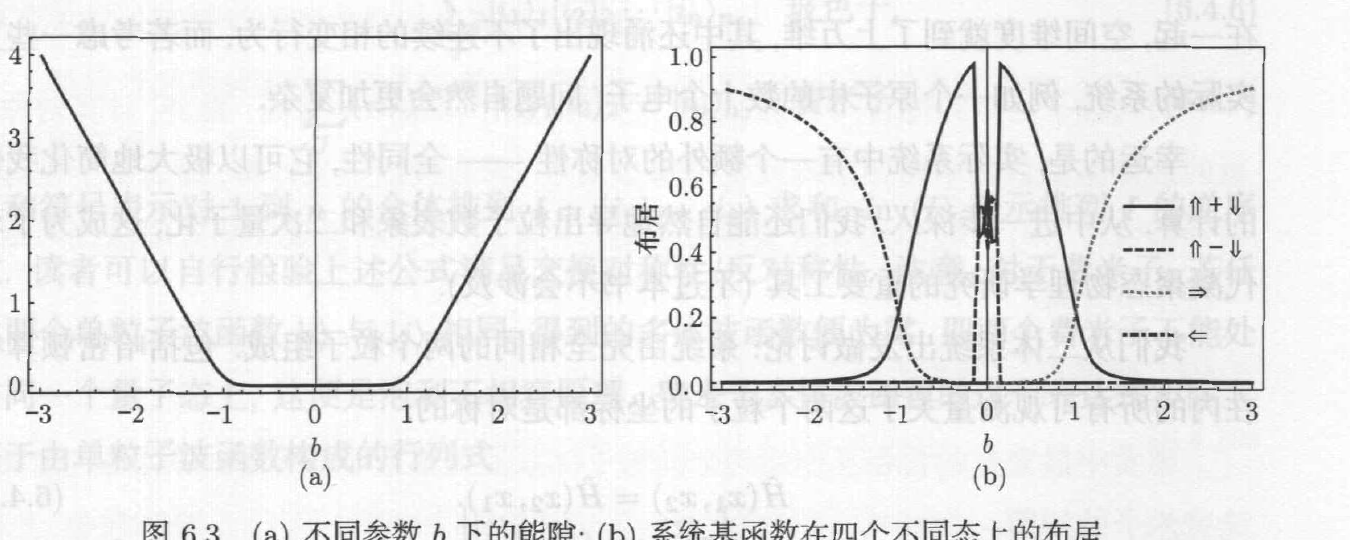
\includegraphics[width=.94\linewidth]{figures/fig6_3_ising.png}
\caption{(a) 不同参数 $b$ 下的能隙；(b) 系统基函数在四个不同态上的布居}
\label{fig:6-3}
\end{figure}

我们可以继续尝试探究导致相变发生的原因。考虑将算符 $-b\sum_{j=1}^{N}\sigma_x^{(j)}$ 作用在 $|\psi_\uparrow\rangle$ 上\jiaokan{原印本此处求和指标写作 $j$，但算符上标仍误写为 $k$。求和中的单体算符应随哑指标变化，故改为 $\sigma_x^{(j)}$；这也与紧随其后的 (6.3.15) 式一致。}，得到的波函数是全部 $N-1$ 个自旋朝上、一个自旋朝下的组态的叠加：
\begin{equation}
 -b\bigl(|\downarrow\uparrow\uparrow\cdots\uparrow\rangle+|\uparrow\downarrow\uparrow\cdots\uparrow\rangle+|\uparrow\uparrow\downarrow\cdots\uparrow\rangle+\cdots\bigr).
\tag{6.3.14}
\end{equation}
\footnote{请读者思考：为何不取 $|\psi_\uparrow\rangle$ 作为初始迭代向量？}

\originalpage{241}{226}
每作用一次，都会让其中某一个自旋发生翻转。那么，至少需要作用 $N$ 次，才能将 $|\psi_\uparrow\rangle$ 和 $|\psi_\downarrow\rangle$ 联系起来：
\begin{equation}
 \langle\psi_\downarrow|\frac{\left(-b\sum_{k=1}^{N}\sigma_x^{(k)}\right)^N}{N!}|\psi_\uparrow\rangle\propto b^N.
\tag{6.3.15}
\end{equation}
以上讨论告诉我们几个事实：在 $b$ 非零的情况下，$|\psi_\uparrow\rangle$ 和 $|\psi_\downarrow\rangle$ 两个态存在耦合，按照简并微扰论，它们会重新组合成两个能量不同的能级。在 $|b|<1$ 的情况下，这个耦合是非常弱的，因此劈裂产生的带隙非常小。而当 $|b|>1$ 时，耦合又非常强，微扰论失效。那么当 $|b|$ 连续地从小于一增长到大于一时，系统的行为自然会发生突变。我们将相变和幂函数 $x^N$ 在 $N\to\infty$ 时的不一致连续性联系了起来。

图 6.3(b) 中的四条曲线分别给出了系统基态波函数在 $(|\psi_\uparrow\rangle+|\psi_\downarrow\rangle)/\sqrt2$、$(|\psi_\uparrow\rangle-|\psi_\downarrow\rangle)/\sqrt2$、$|\psi_\rightarrow\rangle$ 和 $|\psi_\leftarrow\rangle$ 四个态上的布居。$b=0$ 附近的跳变来源于此处带隙过小，数值算法难以区分两个近简并态。波函数的过渡区域相比本征能量而言更宽，这个结果与 3.4 节最后提到过的用瑞利商估计本征值的精度相比波函数更高这一事实具有类似的缘由：当波函数受到一个扰动时，本征能量的变化正比于波函数变化的平方。

% R19 extends through source scan p.241 / printed p.226, completing Section 6.3.

\section{全同粒子：单组态与多组态计算}

上一节中，我们见识过了量子多体系统的复杂性：仅仅是将十来个二能级系统放在一起，空间维度就到了上万维，其中还涌现出了不连续的相变行为。而若考虑一些更实际的系统，例如一个原子中的数十个电子，问题自然会更加复杂。

幸运的是，实际系统中有一个额外的对称性——全同性，它可以极大地简化我们的计算。从中进一步深入，我们还能自然地导出粒子数表象和二次量子化，这成为了现代凝聚态物理学研究的重要工具（不过本书不会涉及）。

我们从二体系统出发做讨论。系统由完全相同的两个粒子组成，包括哈密顿算符在内的所有可观测量关于这两个粒子的坐标都是对称的：
\begin{equation}
 \hat H(x_1,x_2)=\hat H(x_2,x_1).
\tag{6.4.1}
\end{equation}
这里 $x_k$ 可以单指粒子的空间坐标，也可能包含其自旋等其他自由度的信息。我们定义交换算符 $\hat P$：
\begin{equation}
 \hat P|\alpha\rangle_1|\beta\rangle_2=|\beta\rangle_1|\alpha\rangle_2,
\tag{6.4.2}
\end{equation}
用以交换两个粒子的态。由于哈密顿算符的交换对称性，其与交换算符对易：
\begin{equation}
 [\hat H,\hat P]=0.
\tag{6.4.3}
\end{equation}

\originalpage{242}{227}
通过与 5.2 节中相类似的讨论我们可以知道，哈密顿量 $\hat H$ 的本征函数一定也是交换算符 $\hat P$ 的本征函数。而注意到交换两次将回到自身，因此交换算符的平方是单位算符：
\begin{equation}
 \hat P^2=\hat I,
\tag{6.4.4}
\end{equation}
则其本征函数的本征值为 $\pm1$。其相应本征函数具有如下形式：
\begin{equation}
 |\alpha\rangle_1|\beta\rangle_2\pm|\beta\rangle_1|\alpha\rangle_2.
\tag{6.4.5}
\end{equation}
这样，两个相同粒子组成的量子态可以分成两类：一类在交换操作下不变，而另一类在交换操作下变号。这个划分是不会随着幺正演化或测量而改变的，具有一类交换对称性的量子态始终会保持该对称性。那么，我们可以干脆将交换对称性不同的两类量子态视作两种不同的粒子，尽管它们其他物理属性可能相同。

令人惊讶的是，实验结果告诉我们，不存在其他物理属性相同，而只有交换对称性不同的粒子，这个交换对称性也不会随体系内同类粒子数的增加而改变。我们将交换操作下波函数不变的粒子称作玻色子，交换操作下波函数变号的粒子称作费米子。

上述的讨论可以扩展到任意粒子数的情况。考虑由 $n$ 个全同粒子组成的系统，在 $|1\rangle$ 态上有一个粒子、$|2\rangle$ 态上有一个粒子、$\cdots$、$|n\rangle$ 态上有一个粒子\footnote{由于全同性，我们没法说第几个粒子处在某个态上。}。那么分别对于玻色子和费米子，这个系统（未归一化的）多体波函数可以由下述公式给出：
\begin{equation}
 \sum_I |i_1\rangle_1|i_2\rangle_2\cdots|i_n\rangle_n,
 \qquad \text{玻色子},
\tag{6.4.6}
\end{equation}
\begin{equation}
 \sum_I(-1)^{\operatorname{Inv}(I)}|i_1\rangle_1|i_2\rangle_2\cdots|i_n\rangle_n,
 \qquad \text{费米子}.
\tag{6.4.7}
\end{equation}
求和符号表示对 $1$ 到 $n$ 的全体排列 $I=(i_1i_2\cdots i_n)$ 求和，$\operatorname{Inv}(I)$ 表示排列 $I$ 的逆序数。读者可以自行检验上述公式满足交换对称性/反对称性。注意，对于费米子，若任意两个单粒子波函数 $|i\rangle$ 与 $|j\rangle$ 相同，得到的多体波函数便为零，即两个费米子不能处在同一个量子态上，这便是 Pauli 不相容原理。费米子多体波函数的这个表达式实际上等于由单粒子波函数构成的行列式
\begin{equation}
 \begin{vmatrix}
 |1\rangle_1&|1\rangle_2&\cdots&|1\rangle_n\\
 |2\rangle_1&|2\rangle_2&\cdots&|2\rangle_n\\
 \vdots&\vdots&\ddots&\vdots\\
 |n\rangle_1&|n\rangle_2&\cdots&|n\rangle_n
 \end{vmatrix},
\tag{6.4.8}
\end{equation}
称为 Slater 行列式（Slater determinant）。注意，Slater 行列式仅是一种构造费米子多体波函数的可能方案，实践中也存在其他构造满足反对称条件波函数的方法。

\originalpage{243}{228}
全同性让多体问题可以得到极大的化简。考虑由 $n$ 个全同粒子组成的系统，单粒子的波函数用 $m$ 维的基组展开，若不考虑全同性，则 $n$ 粒子波函数的基函数有 $m^n$ 个：
\begin{equation}
 |i_1i_2\cdots i_n\rangle\sim |i_1\rangle_1|i_2\rangle_2\cdots|i_n\rangle_n,
 \qquad i_1,i_2,\ldots,i_n\in\{1,2,\ldots,m\}.
\tag{6.4.9}
\end{equation}
如果这些粒子是全同玻色子呢？出于交换对称性，通过粒子间相互“交换位置”所构成的态将与原来相同。例如下面的多体波函数都代表同一个态：
\begin{equation}
 |1223\rangle=|2123\rangle=|3122\rangle=\cdots.
\tag{6.4.10}
\end{equation}
借助排列组合的知识可以证明，在这种意义下，真正互不相同的基函数个数只有
\begin{equation}
 \binom{n+m-1}{n}=\frac{(n+m-1)!}{n!(m-1)!}.
\tag{6.4.11}
\end{equation}
费米子的情形是类似的，下面这些波函数都代表着相同的态：
\begin{equation}
 |1234\rangle=-|2134\rangle=|4321\rangle=\cdots.
\tag{6.4.12}
\end{equation}
与玻色子不同的是，出于 Pauli 不相容原理，诸如 $|1223\rangle$ 这样的态是不会出现的。这些使得全同费米子体系独立的基函数个数更少，其数量为
\begin{equation}
 \binom{m}{n}=\frac{m!}{n!(m-n)!}.
\tag{6.4.13}
\end{equation}
引入粒子的全同性后，问题的维度大大降低了，但依旧非常高。此外，计算对称化后的多体基函数的哈密顿矩阵元也没那么简单：若直接按定义计算，那么每个矩阵元展开都包含 $(n!)^2$ 项，这是没法直接处理的。本节中，我们将简要介绍处理这些问题的一些基本方案。

\subsection{Hartree--Fock 近似}

现实中最常见的含相互作用的全同粒子体系就是多电子体系了，因而我们先来讨论费米子的问题。

$n$ 个全同费米子用 $m$ 个单粒子基组展开，会得到 $\binom{m}{n}$ 个多体基组。如果 $m=n$，我们便只剩下了一个基组，这极大地简化了问题：体系只有一个本征态，即该多体基函数 $|\psi\rangle$，相应本征能量为哈密顿量在基函数下的期望值：
\begin{equation}
 E=\langle\psi|\hat H|\psi\rangle.
\tag{6.4.14}
\end{equation}
这被称为 Hartree--Fock（HF）近似。当然，此时这 $m$ 个单粒子基函数就不能随随便便设置了，我们必须小心选取使得多体基函数尽可能接近真实的本征态。根据 5.4 节中关于 \rusname{Галёркин} 法的讨论，当我们限定矢量的选取于某个子空间时，这个子空间内的约束极值问题将近似给出原问题本征态和本征能量。那么我们需要做的便是调整 $\psi$ 使 $E$ 取得极值，就能得到这种近似下对本征能量 $E_i$ 最好的估计值。

\originalpage{244}{229}
在继续进行下去前，我们需要知道如何计算 $E$。全同粒子的哈密顿算符一般由单体算符和两体算符构成：
\begin{equation}
 \hat H=\sum_{k=1}^{n}\hat h_k+\frac12\sum_{k\ne l}\hat v_{kl}.
\tag{6.4.15}
\end{equation}
这里的 $1/2$ 因子来自求和式中两两间的相互作用被重复计算了一次。单体算符只能将两个相同下标的单粒子态联系在一起，因此 (6.4.7) 式中任意两项关于 $\hat h_i$ 的内积都是零，非零的只有对角项
\begin{equation}
 \langle\cdots i_k\cdots|\hat h_k|\cdots i_k\cdots\rangle=\langle i_k|\hat h|i_k\rangle,
\tag{6.4.16}
\end{equation}
最后得到
\begin{equation}
 \left\langle\psi\left|\sum_{k=1}^{n}\hat h_k\right|\psi\right\rangle=\sum_{i=1}^{n}\langle i|\hat h|i\rangle,
\tag{6.4.17}
\end{equation}
等于单粒子算符对所有单粒子态期望值之和。

随后考虑两体算符。两体算符会将两个不同下标的单粒子态联系在一起，那么我们需要考虑
\begin{equation}
 \langle\cdots i_k\cdots i_l\cdots|\hat v_{kl}|\cdots i_k\cdots i_l\cdots\rangle
 =\langle i_ki_l|\hat v|i_ki_l\rangle,
\tag{6.4.18}
\end{equation}
以及
\begin{equation}
 \langle\cdots i_l\cdots i_k\cdots|\hat v_{kl}|\cdots i_k\cdots i_l\cdots\rangle
 =\langle i_li_k|\hat v|i_ki_l\rangle
\tag{6.4.19}
\end{equation}
两项，最后得到
\begin{align}
 \left\langle\psi\left|\sum_{k\ne l}\hat v_{kl}\right|\psi\right\rangle
 &=\sum_{k\ne l}\bigl(\langle i_ki_l|\hat v|i_ki_l\rangle-\langle i_li_k|\hat v|i_ki_l\rangle\bigr)\notag\\
 &=\sum_{i\ne j}\bigl(\langle ij|\hat v|ij\rangle-\langle ij|\hat v|ji\rangle\bigr).
\tag{6.4.20}
\end{align}
这两项分别被称为 Hartree 项和 Fock 项，也称库仑项和交换项。注意到 $i=j$ 时两项相互抵消，因此求和中 $i\ne j$ 的约束可以去除。推导过程中我们始终假定了 $\{|i\rangle\}$ 是一组正交归一基。

\originalpage{245}{230}
那么问题便归结为求解哈密顿量期望值在约束 $\langle i|j\rangle=\delta_{ij}$ 下的极小值。借助拉格朗日乘子消去约束，目标函数写作
\begin{align}
 G&=\langle\hat H\rangle-\sum_{i,j}\lambda_{ij}(\langle i|j\rangle-\delta_{ij})\notag\\
 &=\sum_{i=1}^{n}\langle i|\hat h|i\rangle
 +\frac12\sum_{i,j}\bigl(\langle ij|\hat v|ij\rangle-\langle ji|\hat v|ij\rangle\bigr)
 -\sum_{i,j}\lambda_{ij}(\langle i|j\rangle-\delta_{ij}).
\tag{6.4.21}
\end{align}
为明确起见，我们假定 $n$ 维基组 $\{|i\rangle\}$ 可以用另一基组 $\{|b_\alpha\rangle\}$ 做展开：
\begin{equation}
 |i\rangle=\sum_\alpha c_{i\alpha}|b_\alpha\rangle,
\tag{6.4.22}
\end{equation}
这样目标函数就可以写成系数矩阵 $c_{i\alpha}$ 的一个四次函数，
\begin{align}
 G={}&\sum_{i,\alpha,\beta}h_{\alpha\beta}c_{i\alpha}^*c_{i\beta}
 -\sum_{i,j,\alpha,\beta}\lambda_{ij}
 \bigl(c_{i\alpha}^*S_{\alpha\beta}c_{j\beta}-\delta_{ij}\bigr)\notag\\
 &+\frac12\sum_{i,j,\alpha,\beta,\gamma,\delta}
 \bigl(v_{\alpha\beta,\delta\gamma}-v_{\beta\alpha,\delta\gamma}\bigr)
 c_{i\alpha}^*c_{j\beta}^*c_{i\delta}c_{j\gamma},
\tag{6.4.23}
\end{align}
\jiaokan{原印本式 (6.4.23) 的正交归一约束项写作 $c_{i\alpha}^*S_{\alpha\beta}c_{j\beta}-1$。由前式 $\langle i|j\rangle=\delta_{ij}$ 可知，非对角约束应为 0，故此处应为 $c_{i\alpha}^*S_{\alpha\beta}c_{j\beta}-\delta_{ij}$。}
其中
\begin{equation}
 h_{\alpha\beta}\equiv\langle b_\alpha|\hat h|b_\beta\rangle,
 \qquad S_{\alpha\beta}\equiv\langle b_\alpha|b_\beta\rangle,
 \qquad v_{\alpha\beta,\gamma\delta}\equiv\langle b_\alpha b_\beta|\hat v|b_\gamma b_\delta\rangle.
\tag{6.4.24}
\end{equation}
在极值点处，$G$ 对 $c_{i\alpha}^*$ 的微分为零，由此得到三次方程组
\begin{equation}
 \sum_\beta h_{\alpha\beta}c_{i\beta}
 +\sum_{j,\beta,\delta,\gamma}
 \bigl(v_{\alpha\beta,\delta\gamma}-v_{\beta\alpha,\delta\gamma}\bigr)
 c_{j\beta}^*c_{i\delta}c_{j\gamma}
 =\sum_{j=1}^{n}\lambda_{ij}\sum_\beta S_{\alpha\beta}c_{j\beta}.
\tag{6.4.25}
\end{equation}
这个方程组粗看起来不容易下手，但是，如果我们略微轮换一下指标，并定义 Fock 矩阵
\begin{equation}
 (\mathbf F)_{\alpha\beta}=h_{\alpha\beta}
 +\sum_{j,\delta,\gamma}\bigl(v_{\alpha\delta,\beta\gamma}-v_{\delta\alpha,\beta\gamma}\bigr)c_{j\delta}^*c_{j\gamma},
\tag{6.4.26}
\end{equation}
借助单体算符和两体算符的厄米性，以及两体算符的交换对称性 $v_{\alpha\beta,\gamma\delta}=v_{\beta\alpha,\delta\gamma}$，容易检验 $\mathbf F$ 是一个厄米矩阵，这样，原式就可以写成
\begin{equation}
 \mathbf F\bm c_i=\sum_{j=1}^{n}\lambda_{ij}\mathbf S\bm c_j.
\tag{6.4.27}
\end{equation}
这个式子与矩阵 $\mathbf F$ 和 $\mathbf S$ 的广义本征值问题有些类似，只不过出现在等式右端的是 $\lambda_{ij}$ 而不是通常的 $\lambda_i\delta_{ij}$。这个问题不难处理，我们总可以通过 Schur 分解将 $\lambda_{ij}$ 对角化：
\begin{equation}
 \lambda_{ij}=\sum_k U_{ik}\epsilon_k U_{jk}^*.
\tag{6.4.28}
\end{equation}

\originalpage{246}{231}
引入 $d_i\equiv\sum_jU_{ji}^*c_j$，将 (6.4.27) 式写成广义本征值方程的形式：
\begin{equation}
 \mathbf F\bm d_k=\epsilon_k\mathbf S\bm d_k.
\tag{6.4.29}
\end{equation}
此外，可以发现通过一个幺正变换将向量组 $\{\bm c_i\}$ 重新线性组合成 $\{\bm d_i\}$ 不会改变 Fock 矩阵的形式：
\begin{equation}
 \sum_jc_{j\delta}^*c_{j\gamma}
 =\sum_{j,k,l}U_{jk}^*d_{k\delta}^*U_{jl}d_{l\gamma}
 =\sum_jd_{j\delta}^*d_{j\gamma}.
\tag{6.4.30}
\end{equation}
因此，我们总可以通过对向量组重新做线性组合，在不改变待优化的目标函数和约束的前提下将拉格朗日乘子从 $n^2$ 个减少到 $n$ 个，转换为标准的广义本征值问题。在下文中，我们依旧以 $c_i$ 来指代 $d_i$。

到此为止问题似乎已经得到解决了：计算矩阵 $\mathbf F$，求出其 $n$ 个本征值 $\epsilon_i$ 和本征向量 $\bm c_i$，我们就能构造出 Slater 行列式，得到问题的近似解。但是，要计算矩阵 $\mathbf F$，得先知道 $c_i$！这似乎又回到了究竟有鸡还是先有蛋的问题上来了。

好在处理这类问题我们已经很有经验了，那就是迭代。我们先猜测一组在交叠矩阵 $\mathbf S$ 下正交归一的基组 $\{\bm c_j\}$，然后计算矩阵 $\mathbf F$，根据矩阵的本征向量再来构造新的正交基组，如此循环往复。如果最后得到的 $\{\bm c_j\}$ 和 $\{\epsilon_i\}$ 分别收敛到了一个固定的值，我们就求得了问题的解。体系本征态的能量为
\begin{equation}
 \langle\hat H\rangle=\frac12\sum_{i=1}^{n}\bigl(\epsilon_i+\langle i|\hat h|i\rangle\bigr),
\tag{6.4.31}
\end{equation}
这样写是为了省去两体相互作用项的计算。

通常而言，如果我们想要求解体系的基态，那么就让迭代过程中得到的本征值按从小到大取 $\mathbf F$ 的前 $n$ 个本征值；而如果想求激发态，那么可以考虑留下前 $n$ 个本征值中的一个或多个不取，而是使用更高的本征值和相应本征向量来迭代\footnote{请注意，这种激发态求解方案仅在非常局限的情形下适用。}。这个过程中，我们将 $\mathbf F$ 的本征向量称为轨道（orbital），相应本征值称为轨道能量，迭代过程中所选取的轨道称为占据轨道（occupied orbital），而未选取的则称为未占据轨道（unoccupied orbital）。由一组占据轨道构成的一个 Slater 行列式被称为一个组态（configuration）。求解体系本征态的过程即为在事先确定了各轨道的占据情况后，不断修正各轨道的形状以得到自治方程 (6.4.29) 的解。由于在求解过程中 Fock 矩阵决定了占据轨道，而占据轨道又反过来决定了其所感受的有效哈密顿量，从而这套方案也被称为自洽场（self consistent field, SCF）理论。

我们重新回顾一下整个过程。假定基组 $\{|b_\alpha\rangle\}$ 的维度是 $m$，那么原始问题是一个

\originalpage{247}{232}
$\binom{m}{n}$ 维的矩阵本征值问题。在做 Hartree--Fock 近似后，转换成了一个带约束的非线性优化问题，包含有 $nm$ 个变量和 $n(n+1)/2$ 个约束。通过拉格朗日乘子消去约束，并做微分，其转换成一个非线性方程组。这个非线性方程组可以视作一个 $m$ 维矩阵的本征值问题，并且矩阵本身需要通过本征向量自治计算。由于此时需要求解的往往是矩阵最低的若干个能级，从而在进行矩阵对角化时 Lanczos 分解是非常常用的。

原则上讲，求解 Hartree--Fock 方程未必需要引入具体的基组。历史上，Hartree 于 1928 年在不存在任何现代计算机的情况下基于迭代的思想近似解求解了该方程\footnote{Hartree D R. The wave mechanics of an atom with a non-Coulomb central field. \emph{Math. Proc. Camb. Philos. Soc.}, 1928, 24(1): 111.}；而具体基组的引入则归功于 Roothaan 和 Hall 在 1951 年的工作\footnote{Roothaan C C J. New developments in molecular orbital theory. \emph{Rev. Mod. Phys.}, 1951, 23: 69; Hall G G. The molecular orbital theory of chemical valency. VIII. A method of calculating ionization potentials. \emph{Proc. R. Soc. London A}, 1951, 205: 541.}。因而 (6.4.29) 式有时也被称为 Roothaan--Hall 方程。

下一个问题是上文中所说的迭代能否收敛，收敛速度如何。很不幸的是，这样一个简单直接的迭代方案在面临复杂的实际问题时，经常会出现不收敛的情形\footnote{Koutecký J and Bonačić V. On convergence difficulties in the iterative Hartree--Fock procedure. \emph{J. Chem. Phys.}, 1971, 55: 2408.}。如何提高自治方程迭代的收敛性是量子化学的重要课题之一\footnote{感兴趣的读者可以参考综述 Bris C L. Computational chemistry from the perspective of numerical analysis. \emph{Acta Numer.}, 2005, 14: 363.}。

\subsection{数值实验：氦原子}

花了这么长篇幅在抽象的公式推演上之后，让我们来讨论一个具体的例子：最简单的多电子原子——氦原子。在 $c\to\infty$ 的非相对论极限和 $m_e/m_{\mathrm{He}}\to0$ 的固定核近似下，氦原子的哈密顿算符写作
\begin{equation}
 \hat H=\sum_{i=1,2}\left(\frac{p_i^2}{2}-\frac{2}{r_i}\right)+\frac1{r_{12}}.
\tag{6.4.32}
\end{equation}
我们选取了原子单位制 $m_e=\hbar=e^2/(4\pi\epsilon_0)=1$。哈密顿算符第一项对应单粒子算符，由动能算符及电子与氦核的库仑相互作用构成，第二项对应两体相互作用，为两电子之间的库仑相互作用。

将单体波函数用空间波函数和自旋波函数的基组直积 $\{|\psi_\alpha(\bm r)\rangle\otimes|\uparrow\rangle,|\downarrow\rangle\}$ 做展

\originalpage{248}{233}
开，我们可以给出前文中各项矩阵元的具体表达式：
\begin{equation}
 h_{\alpha s_1,\beta s_2}=\delta_{s_1s_2}\int\psi_\alpha^*(\bm r)\left(\frac{p^2}{2}-\frac2r\right)\psi_\beta(\bm r)\,d^3r,
\tag{6.4.33}
\end{equation}
\begin{equation}
 S_{\alpha s_1,\beta s_2}=\delta_{s_1s_2}\int\psi_\alpha^*(\bm r)\psi_\beta(\bm r)\,d^3r,
\tag{6.4.34}
\end{equation}
\begin{align}
 v_{\alpha s_1,\beta s_2;\gamma s_3,\delta s_4}
 &=\delta_{s_1s_3}\delta_{s_2s_4}
 \int\psi_\alpha^*(\bm r_1)\psi_\beta^*(\bm r_2)\frac1{r_{12}}
 \psi_\gamma(\bm r_1)\psi_\delta(\bm r_2)\,d^3r_1d^3r_2\notag\\
 &=\delta_{s_1s_3}\delta_{s_2s_4}u_{\alpha\beta;\gamma\delta}.
\tag{6.4.35}
\end{align}
其中 $s$ 为自旋指标。据此我们可以理解两体相互作用张量 $u_{\alpha\beta;\gamma\delta}$ 的物理含义：它给出了电荷密度分布 $\rho_1(\bm r)=\psi_\alpha^*(\bm r)\psi_\gamma(\bm r)$ 与 $\rho_2(\bm r)=\psi_\beta^*(\bm r)\psi_\delta(\bm r)$ 之间的静电势能。我们在 5.4 节中已经给出了这些积分在高斯基函数下的结果。

如果不使用高斯基函数，而使用其他类型的基函数，$u_{\alpha\beta;\gamma\delta}$ 这个双重积分往往会通过如下方式做数值计算：引入静电势场
\begin{equation}
 \phi_{\alpha\gamma}(\bm r')=\int\frac{1}{|\bm r-\bm r'|}\psi_\alpha^*(\bm r)\psi_\gamma(\bm r)\,d^3r,
\tag{6.4.36}
\end{equation}
其满足泊松方程
\begin{equation}
 \nabla^2\phi_{\alpha\gamma}(\bm r)=-4\pi\psi_\alpha^*(\bm r)\psi_\gamma(\bm r),
\tag{6.4.37}
\end{equation}
即静电势场可以通过求解泊松方程给出，这是我们在 5.1 节中已经研究过的问题。得到结果后，再计算一次三重积分即可得到两体相互作用。这个过程通常会比数值计算基函数之间的双积分更稳定高效。

我们再来考虑有关自旋的问题。注意到哈密顿算符与两电子的自旋完全无关，那么其本征函数可以对自旋做分离变量，写成空间波函数和自旋波函数相乘的形式\footnote{在电子数更多的情况下，由于交换对称的要求，这种拆分并不总是可行的，此时往往需要将自旋与空间轨道绑定在一起来求解。}，有
\begin{equation}
 \Psi(\bm r_1,\bm r_2)\sum_{s_1,s_2}a_{s_1,s_2}|s_1s_2\rangle.
\tag{6.4.38}
\end{equation}
其中 $s_1,s_2$ 为自旋指标。由于电子是费米子，我们同时要求两体波函数满足交换反号，那么两体波函数可以按照空间波函数交换反号和自旋波函数交换反号分成两类：
\begin{align}
 \text{单重态（singlet）：}&\quad \Psi(\bm r_1,\bm r_2)=\Psi(\bm r_2,\bm r_1),\qquad a_{s_1s_2}=-a_{s_2s_1},\notag\\
 \text{三重态（triplet）：}&\quad \Psi(\bm r_1,\bm r_2)=-\Psi(\bm r_2,\bm r_1),\qquad a_{s_1s_2}=a_{s_2s_1}.
\tag{6.4.39}
\end{align}
接下来我们对这两种情形分开讨论。将三重态的两体波函数写成单体波函数 Slater 行列式的形式：
\begin{equation}
 \frac1{\sqrt{2!}}
 \begin{vmatrix}
 \psi_1(\bm r_1)|s\rangle_1&\psi_1(\bm r_2)|s\rangle_2\\
 \psi_2(\bm r_1)|s\rangle_1&\psi_2(\bm r_2)|s\rangle_2
 \end{vmatrix}
 =\frac1{\sqrt2}\bigl[\psi_1(\bm r_1)\psi_2(\bm r_2)-\psi_2(\bm r_1)\psi_1(\bm r_2)\bigr]|ss\rangle,
\tag{6.4.40}
\end{equation}

\originalpage{249}{234}
其中 $|s\rangle$ 表示某个指定的自旋态（$|\uparrow\rangle$ 或 $|\downarrow\rangle$）。这个形式意味着我们可以完全不管自旋态，消去了自旋自由度的自治方程写作
\begin{equation}
 \left\{
 \begin{aligned}
 (\mathbf F)_{\alpha\beta}&=h_{\alpha\beta}+\sum_{\delta,\gamma}
 \bigl(u_{\alpha\delta,\beta\gamma}-u_{\delta\alpha,\beta\gamma}\bigr)
 \sum_{i=1,2}c_{i\delta}^*c_{i\gamma},\\
 \mathbf F\bm c_i&=\epsilon_i\mathbf S\bm c_i.
 \end{aligned}
 \right.
\tag{6.4.41}
\end{equation}
而对于单重态，Slater 行列式的形式写作
\begin{equation}
 \frac1{\sqrt{2!}}
 \begin{vmatrix}
 \psi(\bm r_1)|\uparrow\rangle_1&\psi(\bm r_2)|\uparrow\rangle_2\\
 \psi(\bm r_1)|\downarrow\rangle_1&\psi(\bm r_2)|\downarrow\rangle_2
 \end{vmatrix}
 =\psi(\bm r_1)\psi(\bm r_2)\frac{|\uparrow\downarrow\rangle-|\downarrow\uparrow\rangle}{\sqrt2}.
\tag{6.4.42}
\end{equation}
我们仅需要一个空间轨道即可。消去了自旋自由度的自治方程写作
\begin{equation}
 \left\{
 \begin{aligned}
 (\mathbf F)_{\alpha\beta}&=h_{\alpha\beta}+\sum_{\delta,\gamma}u_{\alpha\delta,\beta\gamma}c_\delta^*c_\gamma,\\
 \mathbf F\bm c&=\epsilon\mathbf S\bm c.
 \end{aligned}
 \right.
\tag{6.4.43}
\end{equation}
将矩阵表达式重新写成算符和积分形式会很有趣：
\begin{equation}
 \left[\frac{p^2}{2}-\frac2r+\int d^3r'\frac{|\psi(\bm r')|^2}{|\bm r-\bm r'|}\right]\psi(\bm r)=\epsilon\psi(\bm r).
\tag{6.4.44}
\end{equation}
这看起来像是一个有着“自相互作用”的电子所满足的薛定谔方程。当然，需要注意的是，HF 方法中并不存在“自相互作用”，这里纯粹是因为两条占据轨道的空间波函数完全相同，从而表现出了自相互作用的形式。

接下来的问题便是选取具体的基函数。基函数的选取通常是一个比较复杂的问题，涉及待求解的体系、想获得的物理量以及计算资源的多少等等。不过在这里，我们就采取一个简单的取法：采用四个宽度不同的高斯基函数 $\{e^{-\alpha_i r^2}\mid i=1,2,3,4\}$。我们并没有在指数函数前乘上多项式，这相当于限制了两个电子的轨道都处在 $s$ 态上。我们的目标是求解氦原子的基态能量，因此系数组合 $\{\alpha_i\}$ 的选取应当使得最终算出的基态能量尽可能低。我们在此略去极小化的过程，直接给出氦原子的一个最优取法
\begin{equation}
 \{\alpha_i\}=\{0.298073,1.242567,5.782948,38.474970\}.
\tag{6.4.45}
\end{equation}
借助 5.4 节中关于高斯型轨道积分的结果，并将其代入自治方程 (6.4.43) 式，便可以求解出氦原子单重态的基态能量 $E=-2.8552$。考虑到过程中我们做了如此多的近似，这个结果与实验值 $E_0=-2.9037$ 还是相当接近的。

实践中，人们已经在各种不同的约束下对所有种类的原子找到了最优的高斯型基函数的参数组合，它们被广泛集成在量子化学软件中，同时也可以在互联网上获取\footnote{例如 \texttt{www.basissetexchange.org}.}。这样，在求解分子问题时，将所有原子相应的轨道基组放在一起即可便利地处理。

\originalpage{250}{235}
使用高斯类基函数描述原子分子中的电子波函数虽然简单方便，少许几个基函数就能得到相当不错的近似结果，但却无法准确描述波函数的渐近性质。我们知道，当电子离核足够远时，能量为 $E$ 的束缚态会渐近于指数衰减，
\begin{equation}
 \lim_{r\to\infty}\psi(r)\sim\exp(-\sqrt{-2E}\,r),
\tag{6.4.46}
\end{equation}
而高斯基函数却是呈指数平方衰减的，这使得其无论如何也无法描述离核足够远处波函数的行为。此外，离核非常近的时候也有问题。对于 $s$ 态的电子波函数，在离核足够近时，薛定谔方程写作
\begin{equation}
 -\frac1{2r^2}\frac{d}{dr}\left(r^2\frac{d\psi}{dr}\right)-\frac Zr\psi=0.
\tag{6.4.47}
\end{equation}
注意到 $s$ 态波函数在 $r\to0$ 时不为零，将等式乘 $2r^2$ 做积分，有
\begin{equation}
 -r^2\frac{d\psi}{dr}-Zr^2\psi=0
 \quad\Longrightarrow\quad
 \lim_{r\to0}\frac1\psi\frac{d\psi}{dr}=-Z.
\tag{6.4.48}
\end{equation}
也就是说，波函数的径向导数在核附近不为零，表现为 $\psi(r)\sim\psi(0)(1-Z|r|)$，存在着一个尖点（cusp）。显然，无穷阶可微的高斯类基函数也不可能正确描述这种导数不连续的行为。因此，当我们所需要求解的物理量强烈依赖于波函数在远处或近处的渐近行为时，最好不要使用高斯类基函数。

\subsection{讨论与推广}

在 Hartree--Fock 近似中，我们仅使用了一个 Slater 行列式来描述多体波函数。那么，作为进一步的近似，我们可以使用多个 Slater 行列式，或者说多个组态的线性组合来描述多体波函数。基于这一思路的方法有组态相互作用（configuration interaction, CI）、多组态自洽场（multi-configuration self consistent field, MCSCF）和耦合簇（coupled cluster, CC）等。

如其名字所暗示的，多组态方法相比 HF 更复杂的一点是需要计算不同组态之间的相互作用
\begin{equation}
 \langle\Psi_I|\hat H|\Psi_J\rangle.
\tag{6.4.49}
\end{equation}
如果我们假定构成这些组态的单电子波函数相互之间都是正交的，那么这个矩阵元的计算不会太困难：单电子哈密顿量会在至多有一个单电子波函数不同的组态之间产生非零矩阵元，而双电子相互作用项会在至多有两个单电子波函数不同的组态之间产生非零矩阵元。这些非零矩阵元最终都可以约化到包含两个或四个单电子波函数的积分。对这样一个哈密顿量期望值使用变分法，依赖于 CI 或 MCSCF 方法的选取，能够得到

\originalpage{251}{236}
一个关于组态前系数的线性方程组，抑或是同时包含系数和单电子波函数在内的非线性自治方程组。通过迭代求解该方程组，我们将最后求解得到多电子系统的本征态和本征能量\footnote{关于多组态方法的具体细节，感兴趣的读者可以参考专著 Froese-Fischer C, Brage T, and Jönsson P. \emph{Computational Atomic Structure: An MCHF Approach}. Institute of Physics Publishing, 1997.}。

原则上讲，不断增加组态的数目，我们将逼近多体问题的严格解。将全部单体波函数构造得到的多体组态都纳入考虑范围的方案被称为 full-CI。如果我们之前所讨论过的，此时多体基组的数目为 $\binom{m}{n}$，问题复杂度随着单体基组数目的增长近乎指数增长，是难以用于实践的。

实践中得到更广泛应用的方法是密度泛函理论（density functional theory, DFT），我们将在下一节中具体讨论。

当引入含时哈密顿算符，例如对原子施加强电磁场时，这类基于组态的方法需要同时考虑组态前系数以及构成组态的单电子波函数随时间的变化。如何恰当地处理这类问题依旧属于研究前沿，读者可以自行搜索相应的文献\footnote{如 Anzaki R, Sato T, and Ishikawa K L. A fully general time-dependent multiconfiguration self-consistent-field method for the electron-nuclear dynamics. \emph{Phys. Chem. Chem. Phys.}, 2017, 19: 22008.}。

\section{多电子体系：密度泛函理论}

正如上一节中所讨论的，随着体系粒子数增加，基于 HF 和 CI 方法来获得多体波函数的解变得异常困难。在量子力学诞生的初期，这一困难就被广泛认识。在研究多电子原子和固体等多电子体系时，人们退而求其次，开始探索体系总能量与其电子密度分布之间的关系，也即所谓的能量泛函。这样就可以绕过多电子薛定谔方程的求解，来近似计算系统的性质。基于这个思想的一个典型结果便是 Thomas--Fermi 模型：
\begin{align}
 E_{\mathrm{TF}}[\rho]={}&\frac3{10}(3\pi^2)^{2/3}\int\rho^{5/3}(\bm r)\,d^3r
 +\int\rho(\bm r)v(\bm r)\,d^3r\notag\\
 &+\frac12\iint\frac{\rho(\bm r)\rho(\bm r')}{|\bm r-\bm r'|}\,d^3r\,d^3r'.
\tag{6.5.1}
\end{align}
公式中的三项分别为电子动能、电子在外势场（原子核）中的势能以及电子和电子之间的库仑相互作用。

\subsection{唯一性定理}

这种方案看起来像是某种准经典近似：我们抛弃了多体波函数的相干和纠缠特性，转而考虑经典的电子密度，并将量子的动能项作为某种修正的形式加入。然而，在 1964

\originalpage{252}{237}
年，Hohenberg 和 Kohn 得到了一个重要的结论\footnote{Hohenberg P and Kohn W. Inhomogeneous electron gas. \emph{Phys. Rev.}, 1964, 136: B864.}：只需要考虑电子密度就够了！

\begin{keybox}[定理 6.1（Hohenberg--Kohn 第一定理）]
将多体电子系统置于单体相互作用势场 $v(\bm r)\psi^\dagger(\bm r)\psi(\bm r)$ 中，若其基态 $|\Phi\rangle$ 不简并，那么，不存在两个不同的势函数 $v(\bm r)$（除非仅相差一个常数）能给出相同的基态密度分布 $\rho(\bm r)=\langle\Phi|\psi^\dagger(\bm r)\psi(\bm r)|\Phi\rangle$。
\end{keybox}

\textbf{证明}
采用反证法。假设存在两个不同的外势 $v(\bm r),v'(\bm r)$，它们分别对应不同的哈密顿量 $H$ 和 $H'$，并且给出不同的基态 $|\Phi\rangle,|\Phi'\rangle$，却能给出相同的密度分布 $\rho(\bm r)$。我们有
\begin{align}
 E=\langle\Phi|H|\Phi\rangle
 &<\langle\Phi'|H|\Phi'\rangle
 =\left\langle\Phi'\left|H'+\int[v(\bm r)-v'(\bm r)]\psi^\dagger(\bm r)\psi(\bm r)\,d^3r\right|\Phi'\right\rangle\notag\\
 &=E'+\int[v(\bm r)-v'(\bm r)]\rho(\bm r)\,d^3r.
\tag{6.5.2}
\end{align}
类似地，我们有
\begin{equation}
 E'<E+\int[v'(\bm r)-v(\bm r)]\rho(\bm r)\,d^3r.
\tag{6.5.3}
\end{equation}
两式相加即有
\begin{equation}
 E+E'<E+E',
\tag{6.5.4}
\end{equation}
\jiaokan{原印本式 (6.5.4) 将矛盾式误印为 $E+E'>E+E'$. 由 (6.5.2)--(6.5.3) 两个严格小于号相加，正确结果应为 $E+E'<E+E'$，从而构成矛盾。}
矛盾，假设不成立，故不存在两个不同的势函数能给出同一个电子密度分布。换言之，若给定一个电子密度分布，若存在，则仅存在唯一的势能函数使其为基态密度分布。

既然势函数由电子密度分布唯一地决定，那么包括基态波函数和基态能量在内的一切物理量都由电子密度确定了。原则上讲，存在一个一般性的能量泛函 $E_{\mathrm{HK}}[\rho(\bm r)]$，可以从基态密度分布直接给出基态能量 $E$，称作 Hohenberg--Kohn 泛函。

为了使这个结果实用化，我们需要引入 Levy--Lieb 泛函
\begin{equation}
 E_{\mathrm{LL}}[\rho(\bm r);v(\bm r)]
 =\min_{|\Phi\rangle\to\rho(\bm r)}\langle\Phi|H|\Phi\rangle,
\tag{6.5.5}
\end{equation}
再使 $|\Phi\rangle$ 在给定密度分布 $\rho(\bm r)$ 的情况下取极小值。显然，如果 $\rho(\bm r)$ 是势函数 $v(\bm r)$ 对应的基态密度分布，那么 Levy--Lieb 泛函将给出与 Hohenberg--Kohn 泛函相同的结果。我们知道哈密顿量的基态波函数在满足归一化条件的约束下将会使能量 $\langle\Phi|H|\Phi\rangle$ 取极小。综合这两个结论，可以得到下面的定理。

\begin{keybox}[定理 6.2（Hohenberg--Kohn 第二定理）]
对任意单体相互作用势场 $v(\bm r)\psi^\dagger(\bm r)\psi(\bm r)$，存在能量泛函 $E[\rho(\bm r);v(\bm r)]$，在归一化约束 $\int\rho(\bm r)d^3r=N$ 下，其关于 $\rho(\bm r)$ 变分极值的位置给出了相应的基态电子密度，即
\begin{equation}
 \frac{\delta E}{\delta\rho}=\mu,
\tag{6.5.6}
\end{equation}
这里 $\mu$ 是约束所对应的拉格朗日乘子。
\end{keybox}

\originalpage{253}{238}

\subsection{Kohn--沈吕九方程}

1965 年，Kohn 和沈吕九引入了一组辅助单体波函数 $|\psi_i\rangle=\psi_i(\bm r)^\dagger|0\rangle$，满足正交归一性 $\langle\psi_i|\psi_j\rangle=\delta_{ij}$ 并能给出密度分布 $\sum_{i=1}^{N}|\psi_i(\bm r)|^2=\rho(\bm r)$。他们将能量泛函进一步形式地\mbox{改写成}
\begin{align}
 E[\rho(\bm r);v(\bm r)]={}&-\frac12\sum_{i=1}^{N}\int\psi_i^*(\bm r)\nabla^2\psi_i(\bm r)\,d^3r
 +\int v(\bm r)\rho(\bm r)\,d^3r\notag\\
 &+\frac12\iint\frac{\rho(\bm r)\rho(\bm r')}{|\bm r-\bm r'|}\,d^3r\,d^3r'
 +E_{\mathrm{XC}}[\rho(\bm r)].
\tag{6.5.7}
\end{align}
\jiaokan{原印本式 (6.5.7) 将交换关联泛函写作 $E_{\mathrm{XC}}[\rho;v]$。在 Kohn--沈吕九分解中，外势项 $\int v\rho$ 已单独列出，交换关联泛函属于普适内禀泛函，应写作 $E_{\mathrm{XC}}[\rho]$；这也与随后 $v_{\mathrm{XC}}=\delta E_{\mathrm{XC}}[\rho]/\delta\rho$ 的定义一致。}
这样，整个问题就被形式地写成了类似于单组态 Hartree--Fock 的形式，只是多了一个未知的交换关联项 $E_{\mathrm{XC}}$。

与推导 Hartree--Fock 方程时类似，定义拉格朗日泛函
\begin{equation}
 L=E-\sum_{i,j}\epsilon_{ij}\left(\int\psi_i^*(\bm r)\psi_j(\bm r)\,d^3r-\delta_{ij}\right).
\tag{6.5.8}
\end{equation}
取其变分为 0，
\begin{equation}
 \frac{\delta L}{\delta\psi_i^*(\bm r)}=0,
\tag{6.5.9}
\end{equation}
即可得到
\begin{equation}
 \left[-\frac{\nabla^2}{2}+v(\bm r)+\int\frac{\rho(\bm r')}{|\bm r-\bm r'|}\,d^3r'+v_{\mathrm{XC}}(\bm r)\right]\psi_i(\bm r)
 =\sum_j\epsilon_{ij}\psi_j(\bm r),
\tag{6.5.10}
\end{equation}
其中 $v_{\mathrm{XC}}(\bm r)\equiv\delta E_{\mathrm{XC}}[\rho(\bm r)]/\delta\rho(\bm r)$ 为交换关联能量泛函对密度的微商，称作交换关联势。仿照上一节中的推导，可以得到 Kohn--沈吕九方程：
\begin{equation}
 \left[-\frac{\nabla^2}{2}+v(\bm r)+\int\frac{\rho(\bm r')}{|\bm r-\bm r'|}\,d^3r'+v_{\mathrm{XC}}(\bm r)\right]\psi_i(\bm r)
 =\epsilon_i\psi_i(\bm r).
\tag{6.5.11}
\end{equation}
这同样是一个自治场方程：取定交换关联势后，通过求解本征值方程可以得到单电子轨道 $\psi_i(\bm r)$，从而更新密度分布 $\rho(\bm r)$ 和交换关联势 $v_{\mathrm{XC}}$，实现往复迭代，最终得到自治的结果。慢着，我们是不是还不知道交换关联项和密度分布的泛函关系？

\originalpage{254}{239}
\subsection{交换关联泛函}

事实上，寻找一般的交换关联泛函几乎是不可能完成的任务。幸运的是，对于不少交换关联不强的系统，人们找到了一些简单的近似表达式。最简单的便是基于局域密度近似（local density approximation, LDA）的泛函。顾名思义，LDA 泛函近似假设某个位置 $\bm r$ 的交换关联项仅由此处的电子密度决定，即退化成通常的函数
\begin{equation}
 E_{\mathrm{XC}}^{\mathrm{LDA}}=\int\rho(\bm r)\epsilon_{\mathrm{xc}}(\rho)\,d^3r,
\tag{6.5.12}
\end{equation}
其中 $\epsilon_{\mathrm{xc}}(\rho)=\epsilon_x(\rho)+\epsilon_c(\rho)$ 拆分为交换项
\begin{equation}
 \epsilon_x=-\frac34\left(\frac3\pi\right)^{1/3}\rho(\bm r)^{1/3}
\tag{6.5.13}
\end{equation}
和关联项
\begin{equation}
 \epsilon_c=
 \begin{cases}
 A\ln r_s+B+r_s(C\ln r_s+D)+\cdots, & r_s<1,\\[2mm]
 \dfrac{g_0}{2r_s}+\dfrac{g_1}{2r_s^{3/2}}+\cdots, & r_s\ge1,
 \end{cases}
\tag{6.5.14}
\end{equation}
其中引入了局域有效半径 $r_s=\left(\dfrac3{4\pi\rho}\right)^{1/3}$。其余待定参数原则上可以从理论上确定，也可以通过拟合一些量子系统的数值结果来获得。有了这个具体的泛函形式和参数，前面的 Kohn--沈吕九方程就完全可解了。

除去 LDA 这类泛函仅仅是密度的函数，更高阶的泛函则将考虑密度的梯度、电子的自旋和动能、电子的占据轨道，以及非占据轨道等等。目前被研究和使用的泛函有很多很多。关于交换关联泛函的构造是更加专业的内容，也是前沿的课题，学界将探寻严格交换关联泛函的进程比喻作攀爬“雅各的天梯”：一旦找到了严格的交换关联项，那么便如见到了天堂一般，可以轻松地严格求解各种量子系统。然而这个目标却可望而不可即\footnote{感兴趣的读者，可参考 Medvedev M G, et al. Density functional theory is straying from the path toward the exact functional. \emph{Science}, 2017, 355: 49; Jones R O. Density functional theory: Its origins, rise to prominence, and future. \emph{Rev. Mod. Phys.}, 2015, 87: 897.}。

\subsection{其他讨论}

与 Hartree--Fock 方程的求解相同，数值求解 Kohn--沈吕九方程时同样需要引入一组基函数 $\chi_\alpha(\bm r)$ 用以展开 Kohn--沈吕九轨道：
\begin{equation}
 \psi_i(\bm r)=\sum_\alpha c_{i\alpha}\chi_\alpha(\bm r),
\tag{6.5.15}
\end{equation}

\originalpage{255}{240}
过程与上一节是一致的。实践中较为常用的基组可以分为原子轨道基组和平面波基组两类，而原子轨道基组又可以分为 Slater 型轨道（Slater type orbital, STO）和高斯型轨道两类。Slater 型轨道实际上就是类氢原子的束缚态波函数，其思想与 6.1 节中所讨论的类似，使用无电子相互作用下的本征态来求解带有相互作用的问题，其缺点在于相互作用矩阵元的计算非常困难。而关于平面波基组和高斯型轨道的讨论可以参考 5.4 节。

除了直接采用平面波基组和原子轨道基组外，还存在一些混用的方式来取长补短，从而获得更好的精度和效率。也有一些程序采用物理意义和函数形式更模糊但是数值精度更高的数值基组，例如正交多项式、B 样条函数等等。

与 Hartree--Fock 方程一起，Kohn--沈吕九方程为多体系统精确求解奠定了重要基础，在此基础上结合处理多体量子系统的理论方法可以获得更精确的量子力学解。显然，求解体系的基态能量具有重要的意义，不仅在物理学，在化学中同样如此。因此，1998 年 Kohn 因为其主导建立的密度泛函理论和 Pople 一起分享了当年的诺贝尔化学奖，后者是因其对于 Hartree--Fock 和后 Hartree--Fock 方法中基组和程序等方面的引领性贡献获奖。

除去用于求解量子系统的基态外，密度泛函理论还可以推广到动力学的求解，这得益于另一个唯一性定理\footnote{Runge E and Gross E K U. Density-functional theory for time-dependent systems. \emph{Phys. Rev. Lett.}, 1984, 52: 997.}：将多体电子系统置于含时单体势场 $v(\bm r,t)\psi^\dagger(\bm r)\psi(\bm r)$ 中，给定初态波函数 $|\Phi(t_0)\rangle$，并假定 $v(\bm r,t)$ 在 $t_0$ 处可做泰勒展开，那么，不存在两个不同的 $v(\bm r,t),v'(\bm r,t)$（除非仅相差一个时间函数）使得它们会导致系统相同的密度分布 $\rho(\bm r,t)$。借助完全相同的操作，人们可以引入含时密度泛函（time-dependent density functional theory, TDDFT）来研究系统的演化。当然，困难之处依旧在于如何找到一个恰当的交换关联泛函。通常而言，直接将不含时情况下的交换关联项拿过来，只能对体系略微偏离基态的微扰过程做出较为准确的描述。如何利用含时密度泛函理论计算系统一般性的动力学问题依旧是前沿的研究领域。

\begin{center}
\Large\bfseries 大作业：Bose--Einstein 凝聚体
\end{center}

在 6.4 节中，我们讨论了如何使用 HF 近似来处理全同费米子系统。在此处我们将讨论如何处理全同玻色子系统。玻色子相比费米子的关键区别在于，它无须遵守泡利不相容原理，因此若玻色子之间没有相互作用，在零温下所有的粒子都会处在基态上，这被称为 Bose--Einstein 凝聚（Bose--Einstein condensate, BEC）。这类态的多体波函

\originalpage{256}{241}
数由单体波函数的乘积给出（注意它自动满足交换对称性）：
\begin{equation}
 \Psi(x_1,x_2,\ldots,x_n)=\phi(x_1)\phi(x_2)\cdots\phi(x_n).
\tag{1}
\end{equation}
现在考虑存在相互作用的情形。假设系统由 $n$ 个一维运动的全同玻色子构成，粒子间存在 $\delta$ 函数形式的两两吸引，哈密顿算符写作
\begin{equation}
 \hat H=\sum_{i=1}^{n}\left[-\frac12\frac{\partial^2}{\partial x_i^2}+V(x_i)\right]
 -\frac12g\sum_{i\ne j}\delta(x_i-x_j),\qquad g>0.
\tag{2}
\end{equation}
对于相互作用较弱的情形，上述多体波函数的形式依旧是基态的一个不错的近似。试解答以下问题：
\begin{enumerate}[label=\arabic*.]
\item 证明哈密顿算符在 $|\Psi\rangle$ 下的期望值为
\[
 \langle\Psi|\hat H|\Psi\rangle
 =\int\left[-\frac n2\phi^*(x)\phi''(x)+nV(x)|\phi(x)|^2
 -\frac{n(n-1)}2g|\phi(x)|^4\right]dx.
\]
\item 将上式在单体波函数归一的约束下对 $\phi^*(x)$ 取变分，证明可以得到自治方程
\[
 \left[-\frac12\frac{d^2}{dx^2}+V(x)-g(n-1)|\phi(x)|^2\right]\phi(x)=\epsilon\phi(x),
\]
其被称为非线性薛定谔方程，或 \rusname{Гинзбург--Питаевский}--Gross 方程。
\item 对于 $V(x)=0$ 的情形，上述方程可以通过变换 $x\to\tilde x=g(n-1)x$, $\phi\to\tilde\phi=\phi/\sqrt{g(n-1)}$ 消去三次项前的系数。假定 $\phi(x)$ 是实函数，试选取合适的空间格点或函数基组，数值求解自治方程，给出 $\tilde\phi(\tilde x)$ 的函数图像以及能量 $E$ 的表达式。
\item 现在让我们引入谐振子势 $V(x)=x^2/2$。试给出系统的单粒子的基态能量 $\epsilon$ 和单粒子波函数 $\phi(x)$ 随 $g(n-1)$ 从 0 开始增长而变化的关系图。检验当 $g(n-1)=0$ 时你能得到 $\epsilon=1/2$，以及当 $g(n-1)$ 充分大时可以重现上一问的结果。
\item 对于 $g<0$，即排斥势的情形，方程可以近似求解。忽略动能项，微分方程退化为代数方程，有
\[
 \phi(x)=
 \begin{cases}
 \sqrt{\dfrac{\epsilon-V(x)}{-g(n-1)}},&V(x)<\epsilon,\\[2mm]
 0,&V(x)>\epsilon.
 \end{cases}
\]
随后可以通过归一化条件确定 $\epsilon$。依旧取谐振子势 $V(x)=x^2/2$，试通过求解自治方程，检验当 $-g(n-1)$ 充分大时上述近似是否成立。当 $g(n-1)\lesssim-2$ 时，自治方程解的行为可能会与之前所求得的大不相同，你能否在数值上或物理上给出合理的解释？
\end{enumerate}

% R20 extends through source scan p.256 / printed p.241, completing Chapter 6.
